\documentclass[11pt]{article}
\usepackage[T1]{fontenc}
\usepackage{lmodern}
\usepackage{graphicx}
\usepackage{booktabs}
\usepackage[margin=1in]{geometry}
\usepackage{hyperref}
\usepackage{float}
\usepackage{caption}
\usepackage{microtype}
\usepackage{array}
\usepackage{xcolor}

\hypersetup{colorlinks=true,linkcolor=blue!50!black,citecolor=blue!50!black,urlcolor=blue!60!black}
\newcommand{\dataset}[1]{\texttt{#1}}
\newcommand{\InductiveShortlistN}{25}
\newcommand{\InductiveScoreMin}{0.846}
\newcommand{\InductiveScoreMedian}{0.865}
\newcommand{\InductiveScoreMax}{0.917}
\newcommand{\InductiveLandN}{18}
\newcommand{\InductiveOceanN}{7}
\newcommand{\InductiveMagneticSupportN}{7}
\newcommand{\InductiveMagneticDiscordantN}{2}
\newcommand{\InductiveControlN}{6}
\newcommand{\InductiveControlWarningN}{1}
\newcommand{\InductiveRingFamilyN}{26}
\newcommand{\InductiveRingMemberN}{54}
\newcommand{\InductiveRingPairN}{24}
\newcommand{\InductiveRingTripleN}{2}
\newcommand{\InductiveRegionalFamilyN}{20}
\newcommand{\InductiveRegionalClusteredN}{8}


\title{Arcuate Geometries and Terrestrial Impact Structures:\\An Exploratory Geospatial, Null-Model and Inductive Screening Analysis}
\author{Craig Stone}
\date{22 June 2026}

\begin{document}
\maketitle

\begin{abstract}
Earth's impact record is strongly filtered by erosion, burial and tectonics, but circular morphology alone is not diagnostic of impact. Following French's distinction between candidate detection and geological verification, we analyse updated GeoJSON inventories containing 1,318 arcuate geometries, 80 named African structures (19 confirmed, 40 proposed and 21 discarded in the source review), and a repaired, deduplicated global ``astrobleme'' catalogue of 249 entries, of which 82 carry a local match flag for the Earth Impact Database (EID). Spherical centres and diameters were estimated directly from the arc vertices, and catalogue duplicates and rendering geometries were separated from analytical units. Conservative near-concentric clustering reduces the arcs to 1,292 structure-level units. The upper tails of the arc and EID-matched diameter distributions have maximum-likelihood cumulative exponents of $-2.27$ and $-1.42$, respectively. A fitted multiplicative scale of 9.10 yields a shifted two-sample Kolmogorov--Smirnov statistic of $0.051$ (permutation $p=0.145$). EID-matched centres are closer to arc centres than longitude-rotation nulls, but not closer than proposed catalogue entries under a confidence-label permutation. Circular gravity evidence is enriched over domain-matched rotations (Bouguer and free-air $p=0.0001$), whereas magnetic evidence is not ($p=0.127$). A transparent gravity-first extension selects 25 candidates for review, predicts preservation-dependent follow-up, identifies 26 complete-link nested arcuate families and compares their geometry with 11 published lunar multiring basins and three historical Martian examples. Six endogenic controls include Richat, Pilanesberg and Anton Dohrn; Anton Dohrn itself remains highly ranked. High-priority structures are not enriched on mapped active faults after matching by domain, radius and latitude ($p=0.639$). These outputs sharpen falsifiable review priorities, but support candidate screening rather than confirmation that the arcs are impact-generated rings or preserved distal shock boundaries.
\end{abstract}

\section{Introduction}
Hypervelocity impacts generate shock waves, excavation flow and rapid crater modification. French divides crater formation into contact/compression, excavation and modification stages; the final structure is not a frozen shock front but the product of shock-energy deposition followed by large-scale material flow and gravitational collapse \cite[pp.~17--29]{French1998}. Depending on scale and target properties, the result may be a simple crater, a complex crater with central uplift, a peak-ring basin or a multi-ring basin \cite{French1998,Osinski2022}. Earth's preserved record is incomplete because the near-surface products that carry diagnostic evidence are readily eroded, buried or tectonically disrupted \cite[pp.~28--30]{French1998,Osinski2022}. The 2022 Impact Earth synthesis listed 188 hypervelocity impact craters and 13 additional impact sites lacking documented shock metamorphism, while also emphasizing inconsistencies and incompleteness in the terrestrial record \cite{Osinski2022}.

The motivating hypothesis for this study is that some large arcuate geological traces could preserve annular deformation related to ancient impacts whose central morphology has been removed. This is physically conceivable at basin scale: multi-ring basins contain concentric topographic or fault-bounded rings, and Chicxulub's outer ring faults define a diameter of roughly 180--200~km \cite{French1998,Gulick2013}. The physical interpretation requires care. French shows that peak shock pressure decays rapidly with radial distance, approximately as $R^{-2}$ to $R^{-4.5}$ in the models and observations he reviews. Near the eventual crater rim, pressures fall to roughly 1--2~GPa and the disturbance becomes an elastic or seismic wave; it may produce fracturing, faulting or landsliding, but such effects are not readily distinguishable from ordinary geological deformation \cite[pp.~18--19]{French1998}. Circularity is likewise non-unique: volcanic, diapiric, tectonic, karstic and erosional processes all create circular or arcuate structures, while an impact origin requires diagnostic shock metamorphism, meteoritic material or an extraterrestrial geochemical signature \cite[pp.~97--100]{French1998,FrenchKoeberl2010,Osinski2022}.

We therefore treat the arcuate inventory as an unvalidated candidate set and use ``arcuate geometry'' rather than ``shock boundary'' for the measured objects. The goals are to (i) document the updated data at the correct analytical grain, (ii) compare size distributions without assuming a fixed ring-to-crater multiplier, (iii) test spatial association against explicit null models, and (iv) identify the evidence needed to progress from remote candidate screening to geological confirmation.

Figure~\ref{fig:drake-identification} illustrates the visual-identification context in the Drake Passage region. Candidate circles of multiple diameters were traced where broad, partial arcuate patterns appeared coherent across the regional terrain and bathymetric fabric. The overlays record an interpretive screening step: overlap, apparent nesting and alignment with relief were reasons to retain geometries for comparison, not evidence that the mapped forms share an origin or were produced by impact.

\begin{figure}[H]
  \centering
  \includegraphics[width=0.98\textwidth]{drake3.png}
  \caption{Example of manual identification of arcuate geometries in the Drake Passage region. Gold circles and diameter labels show candidate geometries over a shaded terrain--bathymetry visualization. The dense, overlapping set illustrates the exploratory visual context used to compile candidates; it does not imply that every circle corresponds to an independent geological structure or that any has an impact origin.}
  \label{fig:drake-identification}
\end{figure}

\section{Prior art}
\subsection{Impact recognition and preservation}
French's handbook provides the operational foundation for terrestrial impact recognition. It separates \emph{detection}---by field mapping, remote sensing, drilling or geophysics---from \emph{verification} by shock-metamorphic effects, meteoritic material or a projectile-derived geochemical signature \cite[pp.~97--100]{French1998}. It also describes why preservation state changes the expected observation: fresh craters may retain a rim and ejecta; progressively eroded structures may preserve crater-fill breccias, central uplift or deformation; deeply eroded structures may survive only as patches of unusual rocks and diagnostic microscopic effects \cite[pp.~28--30, 98]{French1998}.

The modern identification framework extends these shock-mineral and field criteria. French and Koeberl \cite{FrenchKoeberl2010} distinguish diagnostic evidence---including planar deformation features with appropriate crystallography, high-pressure mineral polymorphs and impact melt or geochemical signatures---from non-diagnostic circular morphology, brecciation or geophysical anomalies. The later global synthesis by Osinski et al. \cite{Osinski2022} formalizes crater and impact-site categories and documents preservation state, shock effects and impactites. For Africa, Reimold and Koeberl \cite{ReimoldKoeberl2014} review confirmed, proposed and discredited structures and show why geophysical discovery must be followed by petrographic or geochemical confirmation.

\subsection{Shock attenuation, rings and distal effects}
French's physical account distinguishes three phenomena that can otherwise be conflated in a spatial catalogue. First, shock-pressure isobars are initially approximately hemispherical and attenuate rapidly with distance. Second, observable crater rings arise principally during excavation and modification through uplift, collapse and faulting. Third, \emph{distal ejecta} are transported deposits---including shocked grains, spherules, tektites and geochemical anomalies---and are not equivalent to annular bedrock fractures \cite[pp.~18--29, 78, 87--90]{French1998}. Our analysis tests the geometry of possible structural rings; it does not map shock-pressure contours or distal ejecta.

\subsection{Rings and large basins}
Multi-ring morphology is well established on ancient planetary surfaces. French defines multi-ring basins as structures with two or more interior rings in addition to an outer rim, while stressing that their formation remains more complex and uncertain than that of smaller craters \cite[pp.~27--28]{French1998}. Orientale, for example, has a roughly 930~km outer ring and several inner rings, while numerical models link its basin architecture to transient-cavity collapse and target rheology \cite{French1998,Potter2013}. Terrestrial analogues are less straightforward because their upper structural levels are commonly removed or buried. Vredefort has been reconstructed as an originally approximately 250--300~km structure from shock distribution, structural patterns and geophysics \cite{Therriault1997,ReimoldKoeberl2014}. Chicxulub is constrained by seismic, gravity and drilling data and contains a peak ring plus semi-continuous arcuate fault systems \cite{Gulick2013}. These examples show both that impact-related arcs exist and that their dimensions are structure- and definition-dependent; they do not justify a universal tenfold conversion between a listed crater diameter and an outer lineament.

\subsection{Bombardment magnitude and structural inheritance}
The broader motivation is not that every arcuate geometry is an impact artefact, but that a substantial and presently unknown fraction could express long-lived structural inheritance from ancient impacts after recognizable crater morphology and diagnostic near-surface materials have been removed. Under the conditional assumption of a cataclysmic Late Heavy Bombardment and extrapolation of lunar cratering rates to Earth, Ryder and colleagues estimated that Earth could have received at least 22,000 craters larger than 20~km, about 40 basins near 1,000~km and several basins near 5,000~km \cite{Ryder2002,RyderKoeberlMojzsis2000}. These are model-dependent scale estimates, not an inventory or a prior probability that any particular arc is impact-related. The magnitude, duration and even the existence of a narrow late cataclysm remain debated; later syntheses favour a wider range of declining or episodic bombardment histories \cite{FassettMinton2013}.

Large impacts can create crustal-scale faults, brecciation, uplift, melt bodies, permeability and hydrothermal circulation. Modern modelling at Vredefort, for example, supports extensive impact-generated permeability and hydrothermal flow \cite{Marchi2024}. We therefore define the \emph{structural-inheritance hypothesis}: an ancient impact-damaged volume may later be reused opportunistically by tectonic strain, magma ascent, groundwater or hydrothermal flow, surface drainage and erosion, including aeolian modification. The present expression could consequently appear tectonic, volcanic, sedimentary or erosional even if an older impact helped localize it. Persistence of this influence for billions of years, particularly into the mantle, is a hypothesis to be tested rather than an established consequence of impact.

\subsection{Evidence hierarchy for the present study}
Table~\ref{tab:evidence} translates French's candidate/verification framework into the interpretation used here. Morphology and geophysics can rank targets, but material evidence controls confirmation.

\begin{table}[H]
\centering
\caption{Evidentiary role of observations relevant to the arcuate inventory, adapted from French \cite[pp.~97--100, 107--110]{French1998}.}
\label{tab:evidence}
\small
\begin{tabular}{>{\raggedright\arraybackslash}p{0.25\textwidth}>{\raggedright\arraybackslash}p{0.26\textwidth}>{\raggedright\arraybackslash}p{0.39\textwidth}}
\toprule
Observation & Role in this study & Principal limitation or follow-up\\
\midrule
Circular or arcuate morphology & Candidate detection and geometric ranking & Non-unique; compare against calderas, intrusions, diapirs, basins and tectonic structures\\
Gravity or magnetic anomaly & Independent candidate support & No single anomaly is diagnostic; model target geology and preservation state\\
Seismic basin architecture & Test shallow disruption, collapse and possible central uplift & Requires structure-specific interpretation and drilling targets\\
Shatter cones and diagnostic shock microstructures & Geological verification & Requires field exposure, core or archived samples and petrographic confirmation\\
Projectile geochemistry or associated meteorite material & Geological verification & Requires appropriate impactites, contamination control and temporal association\\
\bottomrule
\end{tabular}
\end{table}

\subsection{Size--frequency methods}
Crater size--frequency distributions are often displayed cumulatively, but least-squares fits to binned log--log counts can bias slopes and understate uncertainty. Robbins et al. \cite{Robbins2018} recommend empirical distributions, maximum-likelihood fits and resampling methods. We follow that guidance by showing empirical survival functions, estimating Pareto tails by maximum likelihood and using permutation tests for the cross-catalogue comparison. Because the present catalogues are compilations rather than complete crater counts over a defined survey area, their slopes describe catalogue contents and must not be interpreted as impact fluxes or surface ages.

\section{Data and methods}
\subsection{Datasets and analytical units}
\paragraph{Arcuate geometries.} \dataset{arcuate\_geometries.geojson} contains 1,318 \texttt{MultiLineString} features and 1,290 unique names. The inventory was compiled manually over many weeks by visual inspection of GEBCO terrain. Most traces contain 97 vertices and are extremely close to circles by construction: the median absolute radial deviation is 0.75\% of radius. GEBCO is consequently both the observation surface from which candidates were selected and the source of the terrain measurements used in the morphology ranking. The inventory does not include geological age, lithology, provenance class, interpreter effort or independent evidence for impact. Its features are therefore a manually selected hypothesis set, not independent detections or confirmed shock boundaries.

\paragraph{African structures.} \dataset{african\_impact\_structures.geojson} contains 251 map geometries but only 80 named structures. A structure may be represented by a centre point and one or more minimum/maximum-diameter polygons. We collapse these rendering geometries by name and use the centre record as the analytical unit. The source-review labels yield 19 confirmed, 40 proposed/unconfirmed and 21 discarded structures; 18 confirmed structures have a usable diameter. These labels reproduce the underlying 2014 review rather than asserting current confirmation status \cite{ReimoldKoeberl2014}.

\paragraph{Global astrobleme catalogue.} The original \dataset{astroblemes.geojson} contains 253 source rows assembled from confirmed and possible-impact lists and the African review. An audit found 40 imported diameter errors caused by interpreting hidden Wikipedia sort keys as rendered values; 39 were exact tenfold inflations and Gosses Bluff was stored as 220~km rather than the rendered 32~km. All 40 corrections were verified against a dated source snapshot. Coordinate-template labels were separated from structure identity, and four lower-precedence duplicate records were identified. The row-preserving repair is retained for audit, whereas \dataset{catalog\_repair/astroblemes\_analysis.geojson} contains the 249 unique analytical records used here. Eighty-two carry a local EID-match flag. This flag remains a property of the historical compilation rather than a live status assertion.

\subsection{Spherical geometry and diameters}
For each arcuate feature, vertices were converted to three-dimensional unit vectors. Their normalized vector mean defines a spherical centre. Great-circle distances from that centre were calculated using a mean Earth radius of 6,371.0088~km, and twice the median radial distance defines the characteristic diameter. This avoids the severe dateline and high-latitude errors of longitude/latitude bounding boxes. For African structures, the mean of reported minimum and maximum diameter was used where both were available. Global catalogue diameters use the rendered source value preserved in \texttt{diameter\_raw}; affected geodesic display circles were rebuilt after repair. The original file is unchanged, and a row-level ledger records every correction, source match and duplicate decision.

\subsection{Size distributions}
Empirical survival functions show the fraction of each catalogue with diameter at least $D$. For exploratory tail summaries, the continuous Pareto exponent was estimated by maximum likelihood. The lower cutoff $D_{\min}$ was selected by minimizing the Kolmogorov--Smirnov (KS) distance while retaining at least 25 observations. These estimates are descriptive because catalogue completeness and selection functions are unknown.

To test the earlier fixed-scaling argument, we fitted a multiplier $s$ that minimizes the KS distance between $\log D_{\mathrm{arc}}$ and $\log(sD_{\mathrm{astro}})$. We then permuted the pooled diameters 1,999 times, re-estimated $s$ in every permutation, and compared the observed minimized KS statistic with its null distribution. This accounts for selecting the scale from the same data used in the comparison.

\subsection{Spatial null models}
Arc and catalogue centres were compared by great-circle distance. Two complementary nulls were run with a fixed seed and 9,999 replicates.

\begin{enumerate}
  \item \textbf{Longitude rotation.} A common random longitude offset was added to every EID-matched catalogue centre. This preserves their latitudes and internal longitudinal configuration while breaking alignment with the fixed arc inventory. The statistics were the number of EID matches within 100~km of an arc centre and their median nearest-arc distance.
  \item \textbf{Confidence-label permutation.} The observed catalogue locations were fixed and 82 of the 249 analytical entries were randomly assigned to the ``matched'' group. This tests whether EID-matched entries are more strongly associated with arcs than proposed entries under the composite catalogue's own geographic sampling footprint.
\end{enumerate}

These nulls address spatial coincidence, not geological causation. They cannot correct undocumented feature selection, shared source material or the possibility that known circular structures were deliberately included in both inventories.

\subsection{Bathymetric-source and geophysical screening}
Candidate-centred windows were sampled from the GEBCO 2026 15-arcsecond terrain and Type Identifier (TID) grids \cite{GEBCO2026}, the 2-arcminute WGM2012 Bouguer, free-air, isostatic and gravity-disturbance grids \cite{Bonvalot2012,Balmino2012}, the 2-arcminute EMAG2v3 magnetic anomaly upward-continued to 4~km altitude \cite{Meyer2017}, the 5-arcminute GlobSed total sediment-thickness grid \cite{Straume2019}, and the 1-degree CRUST1.0 model \cite{Laske2013}. CRUST1.0 is retained only as regional context because its cells are too coarse for candidate-scale circularity.

Circular or annular gravity anomalies are physically plausible expressions of impact excavation, collapse, brecciation, melt emplacement, central uplift, basin infill and subsequent burial, because these processes redistribute material density radially. However, comparable anomalies can arise from volcanic, intrusive, sedimentary and tectonic structures. Gravity concordance therefore supports structural follow-up but is not diagnostic of impact origin.

For each continuous field, a Gaussian trend with scale proportional to candidate radius was removed. We measured radial-versus-tangential gradient alignment in a normalized annulus, angular continuity in 36 sectors, annular-gradient enrichment over neighbouring radii, central/annular robust anomaly contrast, valid coverage and diameter in native pixels. Their resolution-weighted combination is a screening ``ring score'', not an impact probability. TID flags were kept categorical: direct and modelled fractions, source diversity, transition density and transition alignment with the candidate annulus were used to estimate source-boundary artefact risk. These evidence channels do not alter the original morphology follow-up score.

No optical or aerial-image measurement contributed to the completed ranking. The generated Sentinel-2 file is a request manifest for future acquisition, not an analysed image dataset. References below to cross-layer support therefore mean terrain, GEBCO source class, gravity, magnetics, sediment context, coarse crustal context and mapped geology or faults; they do not imply optical-image validation.

Two geophysical null designs were run with seed 20260621. First, 19 longitude-rotation locations per candidate preserved latitude and radius and were accepted only when GEBCO TID classified both observed and null windows in the same land/ocean/mixed domain; 9,999 global resamples tested enrichment of median ring score (mean for zero-inflated TID risk). Second, each geophysical score was permuted 9,999 times among candidates within land/ocean/mixed and log-diameter-decile strata. The latter tests cross-layer concordance with the morphology ranking beyond broad domain and scale. Individual candidate $p$ values have a minimum of 0.05 and are treated only as coarse screening diagnostics.

Table~\ref{tab:layer-roles} distinguishes layers that were available for candidate screening from those carried into the final global null tests. Unequal valid counts reflect coverage and resolution rather than a common complete-case cohort.

\begin{table}[H]
\centering
\caption{Role and coverage of the completed screening layers. Candidate-metric counts precede the stricter coverage and resolution checks used by each null.}
\label{tab:layer-roles}
\scriptsize
\resizebox{\textwidth}{!}{%
\begin{tabular}{@{}p{0.20\textwidth}p{0.11\textwidth}rp{0.30\textwidth}p{0.16\textwidth}@{}}
\toprule
Layer & Nominal resolution & Candidate metrics & Role & Final global null reported\\
\midrule
GEBCO terrain & 15 arcsec & 1,318 & Morphology score and candidate-centred terrain & No empirical score null\\
GEBCO TID & 15 arcsec & 1,285 complete rotations & Source-transition artefact risk & Yes\\
WGM Bouguer/free-air & 2 arcmin & 1,256 each & Circular gravity screening & Yes\\
WGM disturbance/isostatic & 2 arcmin & 1,256 each & Supplementary gravity descriptors & No\\
EMAG2v3 & 2 arcmin & 1,256 & Circular magnetic screening & Yes\\
GlobSed & 5 arcmin & 523 & Sediment-thickness context & No\\
CRUST1.0 & 1 degree & regional cells & Coarse crustal context only & No\\
Optical/aerial imagery & not acquired & 0 & Planned manual/automated capture & No\\
\bottomrule
\end{tabular}
}
\end{table}

\subsection{Structure consolidation and active-fault control}
Repeat arc picks were consolidated with score-ordered complete-link clustering. Every pair in a cluster was required to have centre separation no greater than 0.25 times the smaller radius and a radius ratio from 0.67 to 1.50. This prevents transitive chains from merging broad overlaps and preserves near-concentric rings at substantially different scales. We tested strict (0.15; 0.80--1.25) and lenient (0.35; 0.50--2.00) thresholds.

The centre of each structure was compared with 13,696 harmonized active-fault traces from the GEM Global Active Faults Database \cite{StyronPagani2020}. Distances and trace lengths within the candidate radius were calculated in a local azimuthal-equidistant projection. These are tectonic controls, not evidence scores, and do not alter the morphology or geophysical ranking. For a geological null, Tier A/B structures were matched to Tier C/D controls by land/ocean domain, radius quintile and absolute-latitude quartile (with documented relaxation of sparse cells). We drew one control per case with replacement in 9,999 replicates and tested active-fault intersection and radius-normalized proximity. The database is incomplete in several continental regions and does not comprehensively map oceanic faults, so absence of a trace cannot be interpreted as absence of tectonic control.

\subsection{Inductive candidate testing, controls and planetary comparison}
The descriptive and null-model results were extended into a conservative candidate-testing pipeline. A gravity-first review score was calculated as
\[
S_{\mathrm{review}}=0.45S_{\mathrm{morphology}}+0.45S_{\mathrm{gravity}}+0.10(1-R_{\mathrm{TID}}),
\]
where gravity is the available Bouguer/free-air consensus percentile and $R_{\mathrm{TID}}$ is the GEBCO source-transition artefact risk. Missing available components are reweighted rather than replaced by zero. The operational shortlist retains diameters of at least 10~km, TID risk no greater than 0.25 and the first 25 rows after deterministic ranking. Magnetics does not enter the score and is flagged separately as supporting or discordant. This quantity is named a review score rather than an impact score because its components are non-diagnostic.

The endogenic control library combines five supplied polygons---Richat, Jabal Arkanu, Djebel Uweinat, Brandberg/Messum and Pilanesberg---with the mandatory Anton Dohrn volcanic-seamount control. Source names, types and descriptions are preserved; comparator-oriented classes, centres and maximum geodesic radii are derived reproducibly. Candidate/control overlap uses the sum of radii. A size-similarity warning is allowed only within a proximity gate, preventing a distant structure of similar diameter from being treated as a local analogue. The present six controls are deliberately heterogeneous and regionally sparse; they test workflow behaviour but do not represent the full endogenic population.

Nested arcuate families were sought across all 1,318 candidates. Every member pair must have centre separation no greater than 0.25 times the smaller radius, each trace must have angular coverage of at least 0.35, and sorted adjacent radii must differ by a factor of at least 1.2. Connected components are refined into deterministic complete-link groups so transitive chains cannot bypass the adjacent-ratio criterion. These are labelled candidate nested geometries rather than impact ring systems. Separately, the 25 shortlisted candidates were assigned rule-based preservation states from domain, diameter, sediment context and gravity support, and grouped into 500-km regional-proximity families. The rules generate testable acquisition priorities---for example, exposed mapping and petrography versus seismic modelling and drilling---rather than geological diagnoses.

Planetary geometry was added only as an external scale and spacing comparison. The lunar table contains 11 multiring basins and preserves the possible/probable/certain assignments and ring diameters measured from LOLA topography and GRAIL gravity by Neumann et al. \cite{Neumann2015}. A deliberately incomplete historical Mars subset contains Argyre, Isidis and Hellas ring interpretations from Pike and Spudis \cite{PikeSpudis1987}. The full Robbins lunar catalogue is retained separately for large-crater context but is not treated as a multiring classification \cite{Robbins2019}. Similar ring ratios or diameters across bodies are not interpreted as evidence of common origin.

\subsection{Interpretive scope}
The tests are deliberately restricted to French's detection stage. A positive result would identify candidates whose centres or size distributions merit follow-up; it would not verify impact. We do not infer a shock-pressure magnitude from arc diameter, equate arcs with distal ejecta, or assume that every modification-stage ring lies at a fixed multiple of transient- or final-crater diameter.

\section{Results}
\subsection{Updated inventory and size distributions}
The 1,318 arc diameters have a median of 126.0~km, a 95\% empirical interval of 7.5--1,723.1~km and a maximum of 7,262.4~km. Table~\ref{tab:arcs} gives updated bin counts. The old values of 1,153 arcs and ten features above 5,000~km are not reproduced: the current file contains four above 5,000~km.

\begin{table}[H]
\centering
\caption{Updated counts of arcuate geometries by spherical median-radius diameter. Fractions use all 1,318 geometries as the denominator.}
\label{tab:arcs}
\begin{tabular}{lrr}
\toprule
Diameter range (km) & Count & Fraction (\%)\\
\midrule
0--100 & 586 & 44.5\\
100--250 & 311 & 23.6\\
250--500 & 193 & 14.6\\
500--1000 & 130 & 9.9\\
1000--2000 & 74 & 5.6\\
2000--5000 & 20 & 1.5\\
5000--10\,000 & 4 & 0.3\\
$>10\,000$ & 0 & 0.0
\\
\bottomrule
\end{tabular}
\end{table}

Figure~\ref{fig:size} shows different catalogue shapes and completeness limits. Maximum-likelihood fits select an arc tail above 1,080~km ($n=89$) with cumulative exponent $-2.27$, an all-astrobleme tail above 22~km ($n=97$) with exponent $-0.93$, and an EID-matched tail above 20~km ($n=43$) with exponent $-1.42$. These replace both the defective-catalogue fit and the old least-squares slopes near $-0.6$, which were sensitive to import errors and an arbitrarily chosen diameter interval.

\begin{figure}[H]
  \centering
  
\includegraphics[width=0.92\textwidth]{fig_size_distributions.pdf}
  \caption{Empirical diameter survival functions. African records are deduplicated to named structures; the confirmed series has 18 usable diameters. Curves describe these catalogues, not area-normalized crater production.}
  \label{fig:size}
\end{figure}

The best fitted multiplier between all astrobleme and arc diameters is $s=9.10$. After fitting this shift, the KS statistic is 0.051 and does not exceed the relabelled null distribution (permutation $p=0.145$; 1,999 replicates). The corrected analysis therefore does not reject a common distributional shape after multiplicative scaling. This is compatibility with an estimated, catalogue-dependent scale---not confirmation of a universal 9.1- or tenfold physical relation. Catalogue selection, unknown completeness and heterogeneous definitions of crater and outer-ring diameter remain viable explanations.

\subsection{Morphology-ranking calibration}
The morphology score is not equally informative at all scales (Figure~\ref{fig:score-diameter}). For the 48 candidates below 10~km diameter, the median follow-up score is 0.128 and median data-quality weight is 0.215; the median candidate spans only about 15 native GEBCO pixels. From 10 to 1,000~km, median scores remain close to 0.59--0.61. The decline to 0.521 for the 98 candidates at or above 1,000~km identifies a second scale regime in which regional detrending, spherical geometry and the meaning of a single annulus require separate validation. Low scores in the smallest class therefore primarily indicate inadequate resolving power, not geological absence, and the largest class should not be interpreted with the same calibration as intermediate scales.

\begin{figure}[H]
  \centering
  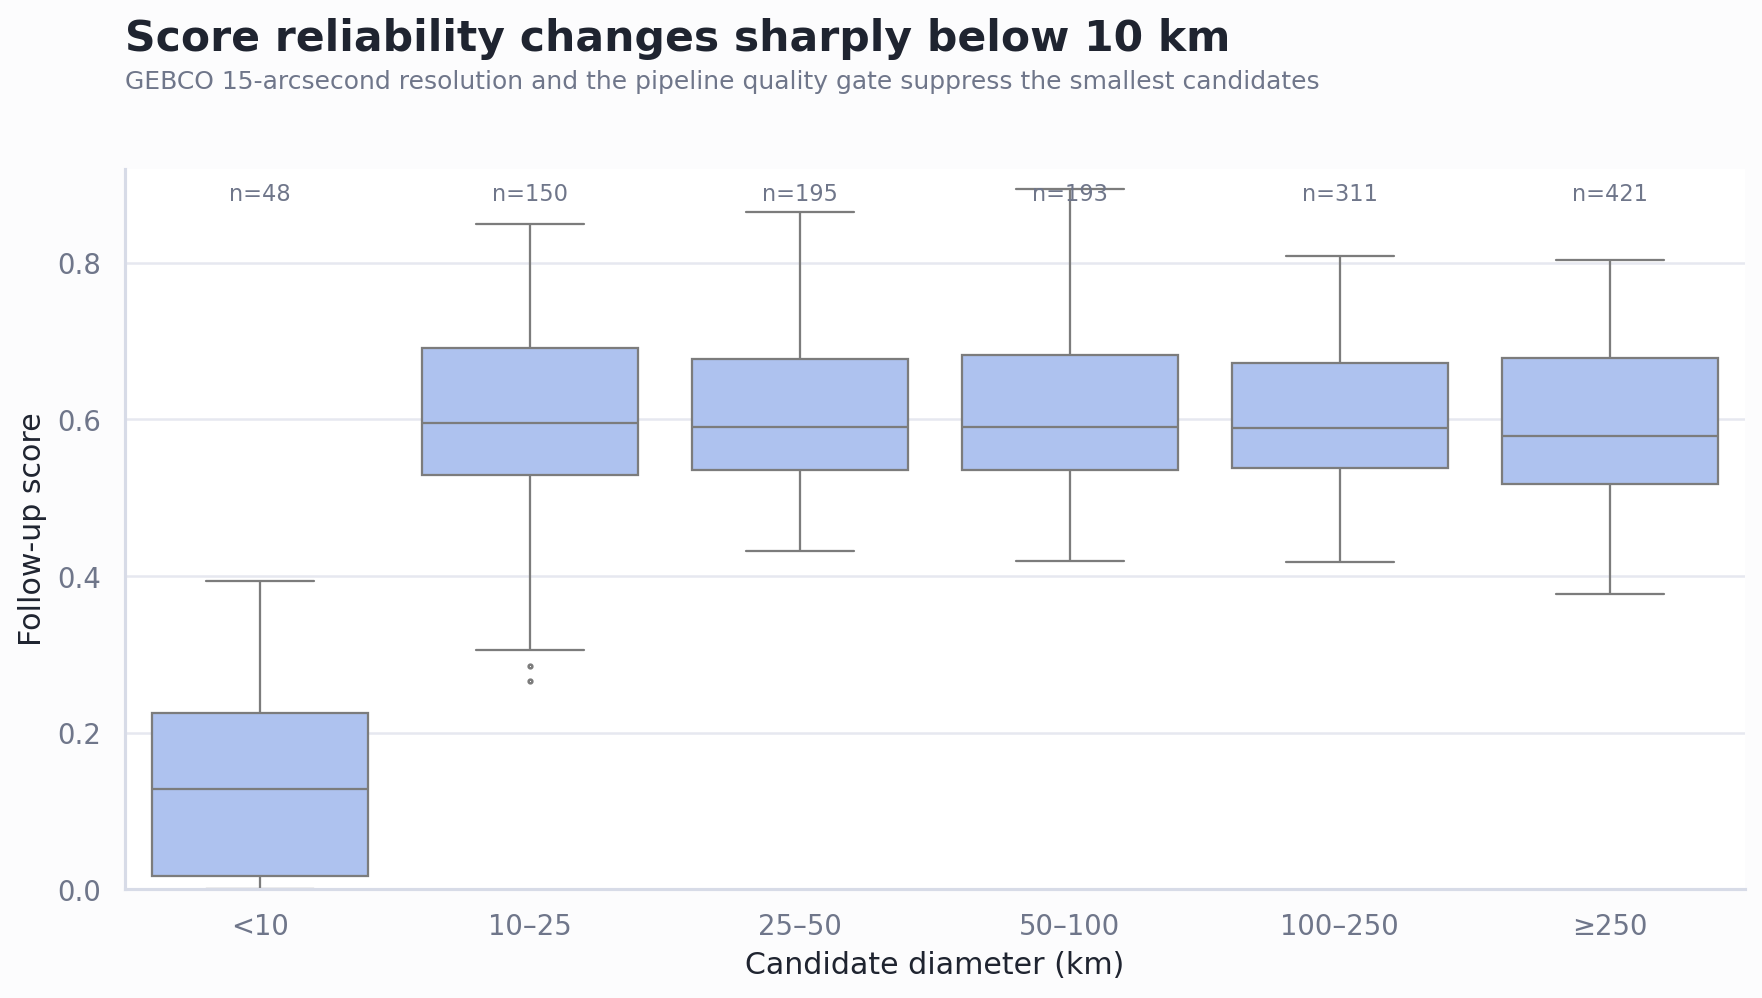
\includegraphics[width=0.96\textwidth]{results_review/charts/score_by_diameter.png}
  \caption{Morphology follow-up score by fitted candidate diameter. The sharp score suppression below 10~km reflects GEBCO resolution and the pipeline quality gate. The plotted $\geq250$~km class combines several large-diameter regimes; the text separately reports the decline at $\geq1,000$~km.}
  \label{fig:score-diameter}
\end{figure}

The score is principally a topographic-circularity ranking. Its strongest rank associations are with composite topography ($\rho=0.854$), annular-peak percentile ($\rho=0.786$), radius agreement ($\rho=0.659$) and angular continuity ($\rho=0.646$; Figure~\ref{fig:score-drivers}). These associations are descriptive decomposition rather than independent predictor importance because the fields are inputs to the composite score. Geological-boundary independence, annular relief and radial alignment have much weaker marginal associations and do not validate impact origin.

\begin{figure}[H]
  \centering
  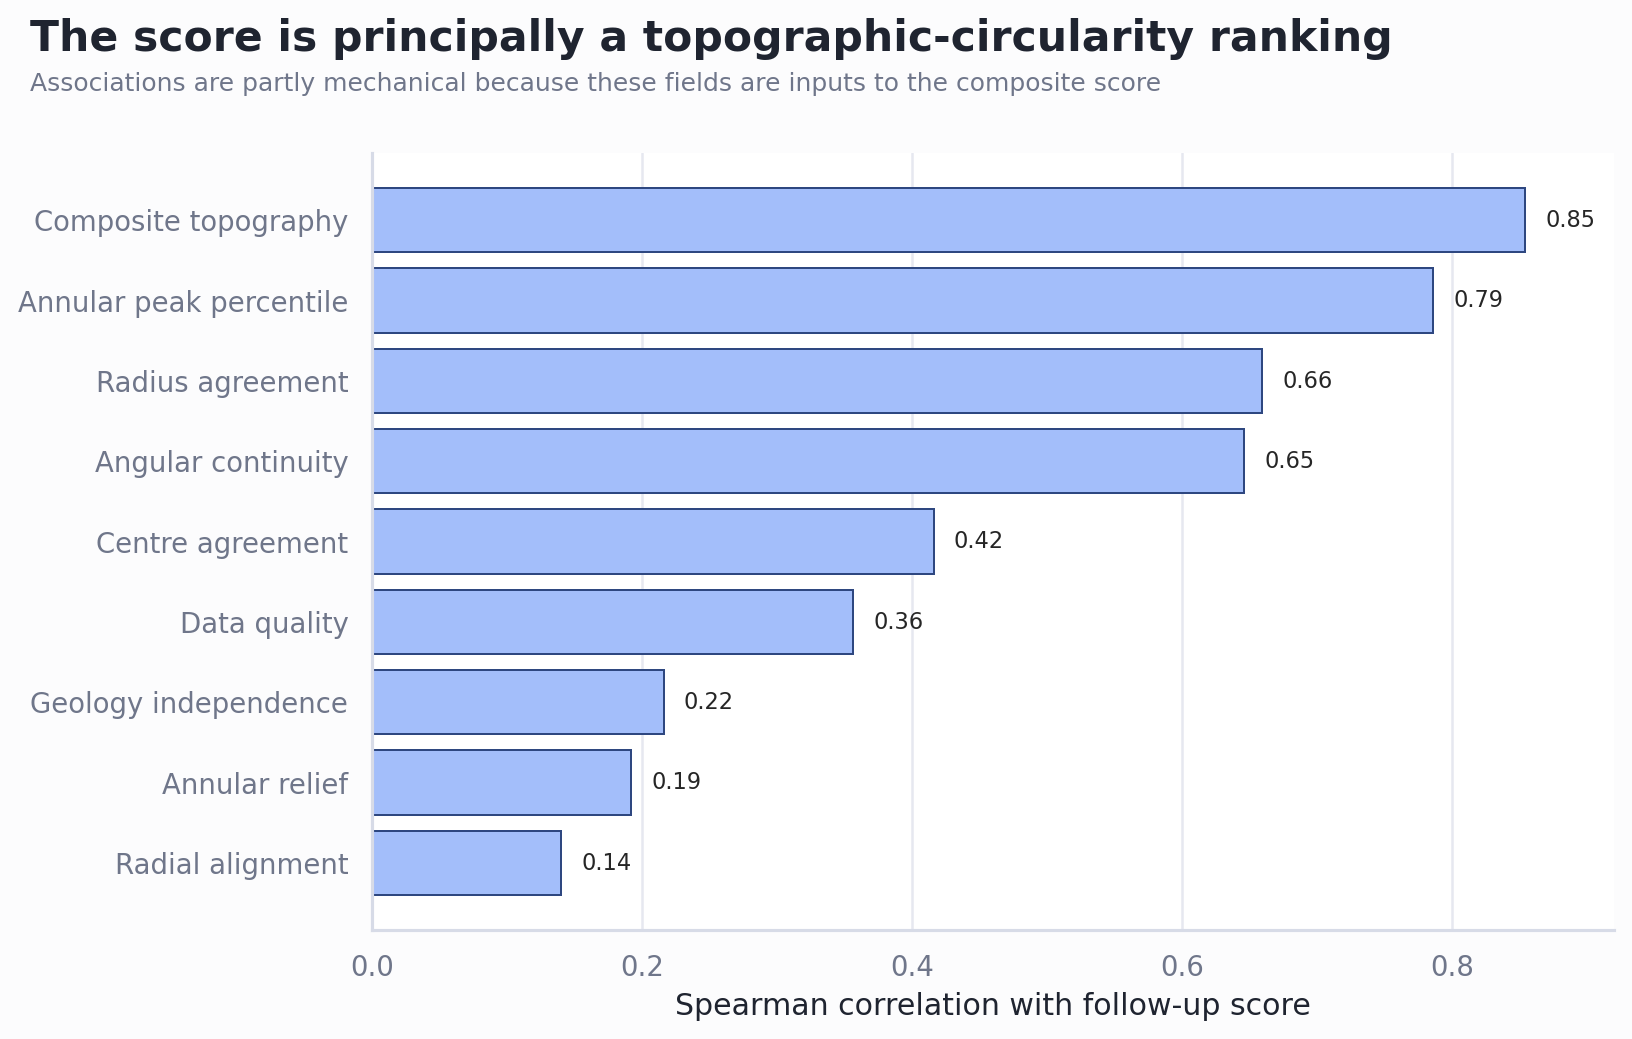
\includegraphics[width=0.92\textwidth]{results_review/charts/score_drivers.png}
  \caption{Spearman associations between component measurements and morphology follow-up score. High values are partly mechanical because the components define the score; this figure explains the ranking rather than validating it against an external outcome.}
  \label{fig:score-drivers}
\end{figure}

\subsection{Spatial distributions and null tests}
The arc inventory is globally distributed but visibly concentrated in particular latitude bands and regions (Figure~\ref{fig:maps}). The composite impact catalogue is also geographically uneven. These patterns make a uniform-on-the-sphere null unsuitable and motivate the constrained rotations and label permutations.

\begin{figure}[H]
  \centering
  
\includegraphics[width=0.96\textwidth]{fig_catalogue_maps.pdf}
  \caption{Updated geometries and catalogue centres. The panels deliberately distinguish raw arcs, EID-matched entries, other composite-catalogue entries and confirmed African structures. Graticules provide location only; no geological base layer is implied.}
  \label{fig:maps}
\end{figure}

Sixteen of the 82 EID-matched entries lie within 100~km of an arc centre, and their median nearest-arc distance is 241.3~km. Both statistics are more extreme than the longitude-rotation null (Table~\ref{tab:nulls}; Figure~\ref{fig:nulls}). However, neither differs significantly from confidence-label permutations within the composite catalogue. Thus the observed proximity is stronger than arbitrary longitudinal alignment but is not specific to the catalogue's EID-matched class.

\begin{table}[H]
\centering
\caption{Spatial null-model results. Brackets give the central 95\% of 9,999 null replicates. One-sided empirical $p$ values include a plus-one correction.}
\label{tab:nulls}
\small
\begin{tabular}{p{0.22\textwidth}p{0.25\textwidth}r>{\raggedright\arraybackslash}p{0.25\textwidth}r}
\toprule
Null & Statistic & Observed & Null median [95\% interval] & $p$\\
\midrule
Longitude rotation & Count within 100 km & 16 & 6 [1, 13] & $0.015$\\
Longitude rotation & Median nearest distance (km) & 241.3 & 379.0 [279.1, 540.0] & $0.005$\\
Confidence-label permutation & Count within 100 km & 16 & 12 [7, 18] & $0.128$\\
Confidence-label permutation & Median nearest distance (km) & 241.3 & 259.1 [214.2, 295.9] & $0.262$
\\
\bottomrule
\end{tabular}
\end{table}

\begin{figure}[H]
  \centering
  
\includegraphics[width=0.94\textwidth]{fig_spatial_nulls.pdf}
  \caption{Null distributions for the count of selected catalogue centres within 100~km of an arc centre. The longitude rotation suggests non-random alignment; the confidence-label permutation shows that this alignment is not enriched among EID-matched entries relative to other entries in the same composite catalogue.}
  \label{fig:nulls}
\end{figure}

\subsection{Bathymetric-source and geophysical null results}
Complete domain-matched rotation sets were obtained for 1,285 candidates; continuous-field tests retained 1,225 candidates after coverage and resolution checks. Mean TID artefact risk is not enriched over matched background ($p=0.9998$), providing no global evidence that the manually selected arcs preferentially follow GEBCO source-class transitions. Bouguer and free-air ring-score medians are enriched over longitude rotations (both $p=0.0001$), but the 4-km upward-continued magnetic ring score is not ($p=0.1268$; Table~\ref{tab:geophysical}).

After stratification by domain and diameter, morphology rank remains positively concordant with Bouguer gravity (Spearman $\rho=0.173$, $p=0.0001$) and free-air gravity ($\rho=0.158$, $p=0.0001$). Magnetic concordance is weak and non-significant ($\rho=-0.017$, $p=0.0717$). Operational review tiers identify 26 Tier A candidates with morphology score at least 0.75, low TID artefact risk and strong Bouguer plus free-air evidence within their domain/size strata, plus six Tier B candidates with partial cross-layer support. Tier A is evenly divided between land and ocean (13 each); Tier B contains five ocean and one mixed-domain case and no land case. This composition can reflect threshold calibration, scale and data availability and is not evidence of geological prevalence. The tiers are review rules rather than significance or probability classes. Candidate-level null $p$ values are quantized at a minimum of 0.05 (including 172 Bouguer and 200 free-air cases at that floor), so they cannot support candidate-level discovery claims or false-discovery-rate control.

\begin{table}[H]
\centering
\caption{Geophysical null results. Null expectation is the resampled mean with central 95\% interval. All tests use seed 20260621 and 9,999 global replicates; longitude rotations use 19 accepted null locations per complete candidate.}
\label{tab:geophysical}
\scriptsize
\begin{tabular}{@{}p{0.17\textwidth}p{0.32\textwidth}r>{\raggedright\arraybackslash}p{0.23\textwidth}r@{}}
\toprule
Null & Statistic & Observed & Null mean [95\% interval] & $p$\\
\midrule
Longitude rotation & TID artefact-risk mean & 0.1137 & 0.1219 [0.1174, 0.1266] & 0.9998\\
Longitude rotation & Bouguer ring-score median & 0.3017 & 0.2706 [0.2663, 0.2747] & 0.0001\\
Longitude rotation & Free-air ring-score median & 0.3262 & 0.2792 [0.2746, 0.2840] & 0.0001\\
Longitude rotation & Magnetic ring-score median & 0.2897 & 0.2866 [0.2812, 0.2922] & 0.1268\\
Stratified permutation & Bouguer--morphology Spearman $\rho$ & 0.1727 & -0.0277 [-0.0653, 0.0091] & 0.0001\\
Stratified permutation & Free-air--morphology Spearman $\rho$ & 0.1584 & -0.0142 [-0.0501, 0.0222] & 0.0001\\
Stratified permutation & Magnetic--morphology Spearman $\rho$ & -0.0173 & -0.0446 [-0.0811, -0.0081] & 0.0717
\\
\bottomrule
\end{tabular}
\end{table}

The category comparison in Figure~\ref{fig:geophysical-comparison} shows why the gravity result merits targeted follow-up. Bouguer and free-air gravity lie beyond their matched-null intervals in the longitude-rotation test and remain positively concordant with morphology after domain/scale stratification (both $p=0.0001$ in both designs). Magnetics does not show the same two-test separation, and TID artefact risk is not enriched. Gravity is therefore the strongest independent remote-sensing lead in the present dataset, while remaining non-diagnostic of impact origin.

\begin{figure}[H]
  \centering
  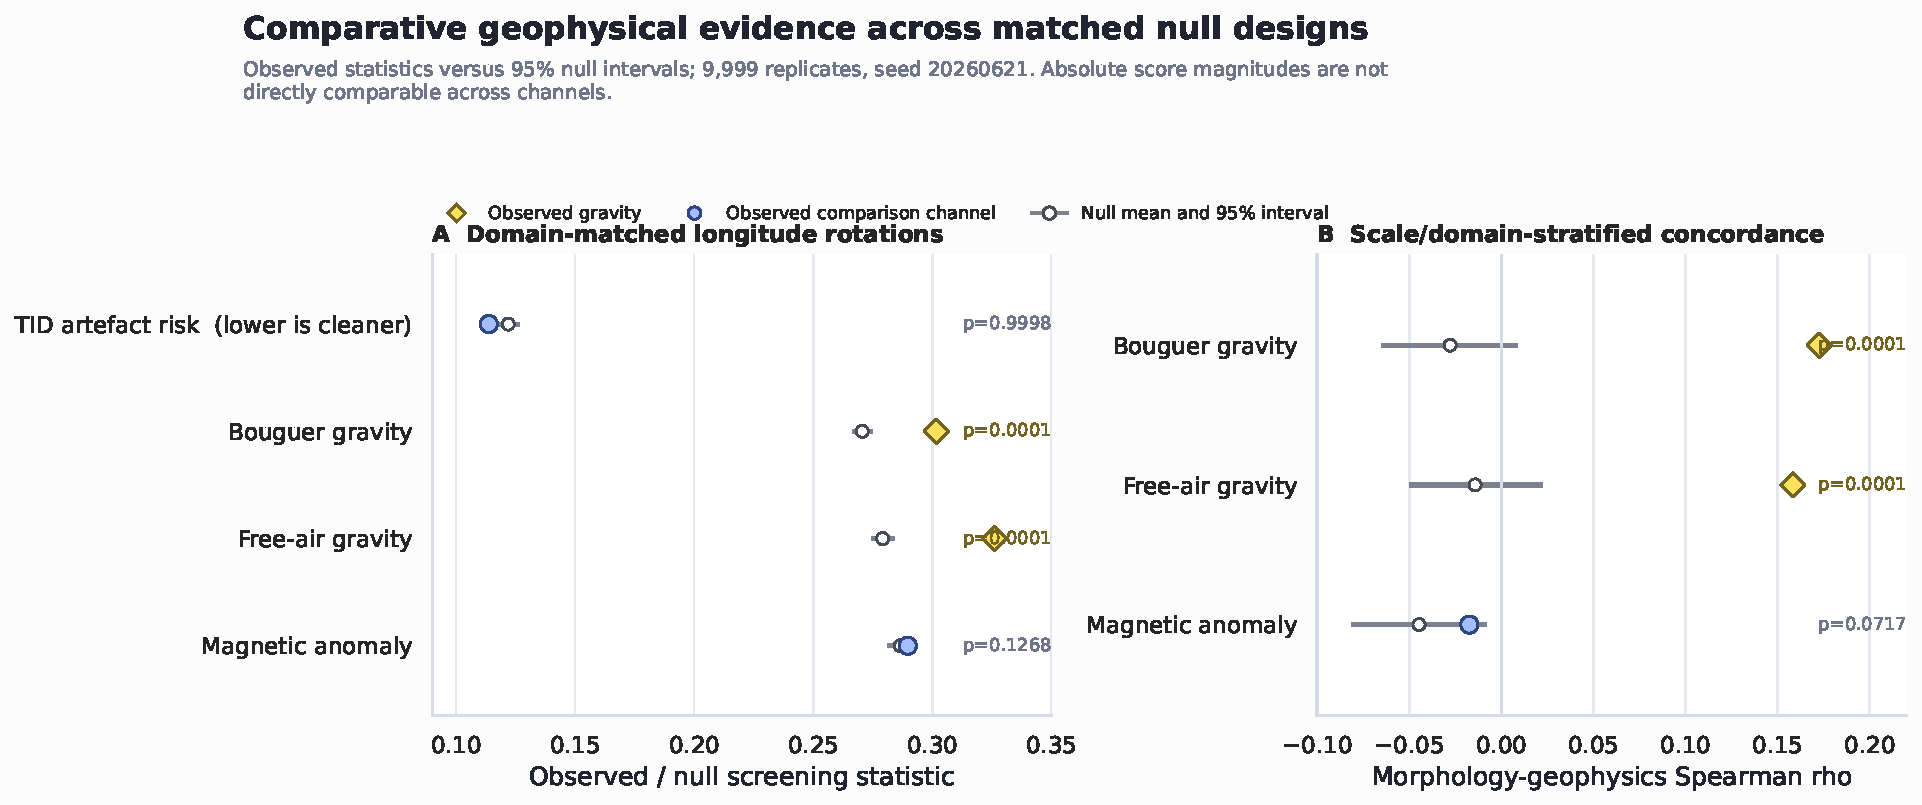
\includegraphics[width=0.98\textwidth]{figure_suite/fig_geophysical_category_comparison.pdf}
  \caption{Comparison of geophysical channels across the two null designs. Filled symbols show observed statistics; open circles and grey bars show null means and central 95\% intervals. Gravity channels are highlighted in gold. Panel A compares observed ring-score summaries with domain-matched longitude rotations; Panel B compares morphology--geophysics concordance with scale/domain-stratified permutations. Absolute score magnitudes differ by channel, so separation from the corresponding null---not raw height---is the relevant comparison.}
  \label{fig:geophysical-comparison}
\end{figure}

Figure~\ref{fig:evidence-matrix} makes the heterogeneity within the operational Tier A/B set explicit. Gravity support is often strong by construction of the tiers, whereas magnetic, boundary and mapped-fault context vary substantially. Anton Dohrn remains a visible reminder that cross-layer coherence is not origin-specific.

\begin{figure}[H]
  \centering
  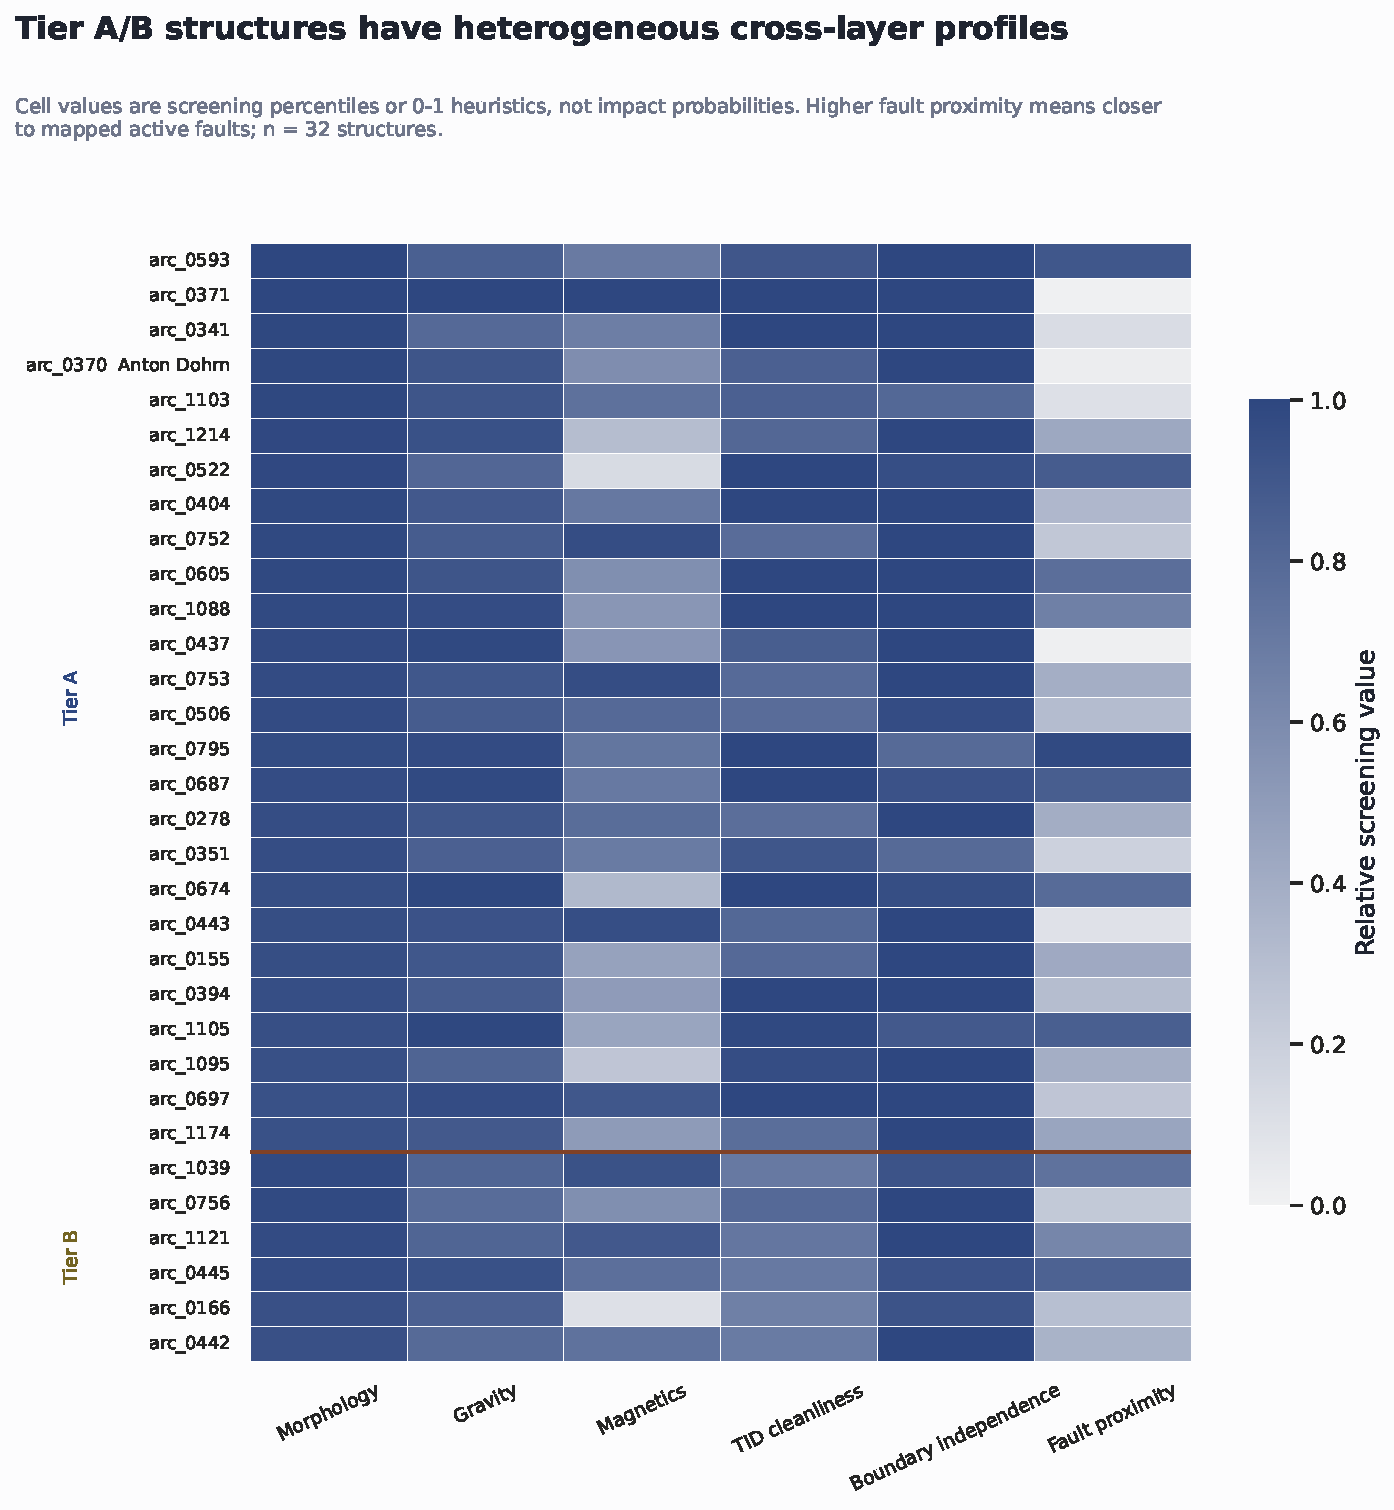
\includegraphics[width=0.82\textwidth]{figure_suite/fig_cross_layer_evidence_matrix.pdf}
  \caption{Cross-layer screening profiles for the 32 structure-level Tier A/B cases. Cells are relative screening percentiles or bounded heuristics, not impact probabilities. Higher fault proximity indicates closeness to mapped GEM active faults. The profile heterogeneity, including the known volcanic Anton Dohrn control, argues against interpreting the tier as a single diagnostic signal.}
  \label{fig:evidence-matrix}
\end{figure}

\subsection{Structure-level catalogue and active faults}
The default consolidation yields 1,292 structure-level units: 25 contain multiple picks and 26 redundant picks are removed. Strict and lenient settings yield 1,309 and 1,279 units, respectively, showing that the conclusion is insensitive to plausible merge thresholds (Figure~\ref{fig:consolidation}). Of the 1,292 units, 222 have a mapped GEM active-fault trace crossing the candidate-radius disk.

\begin{figure}[H]
  \centering
  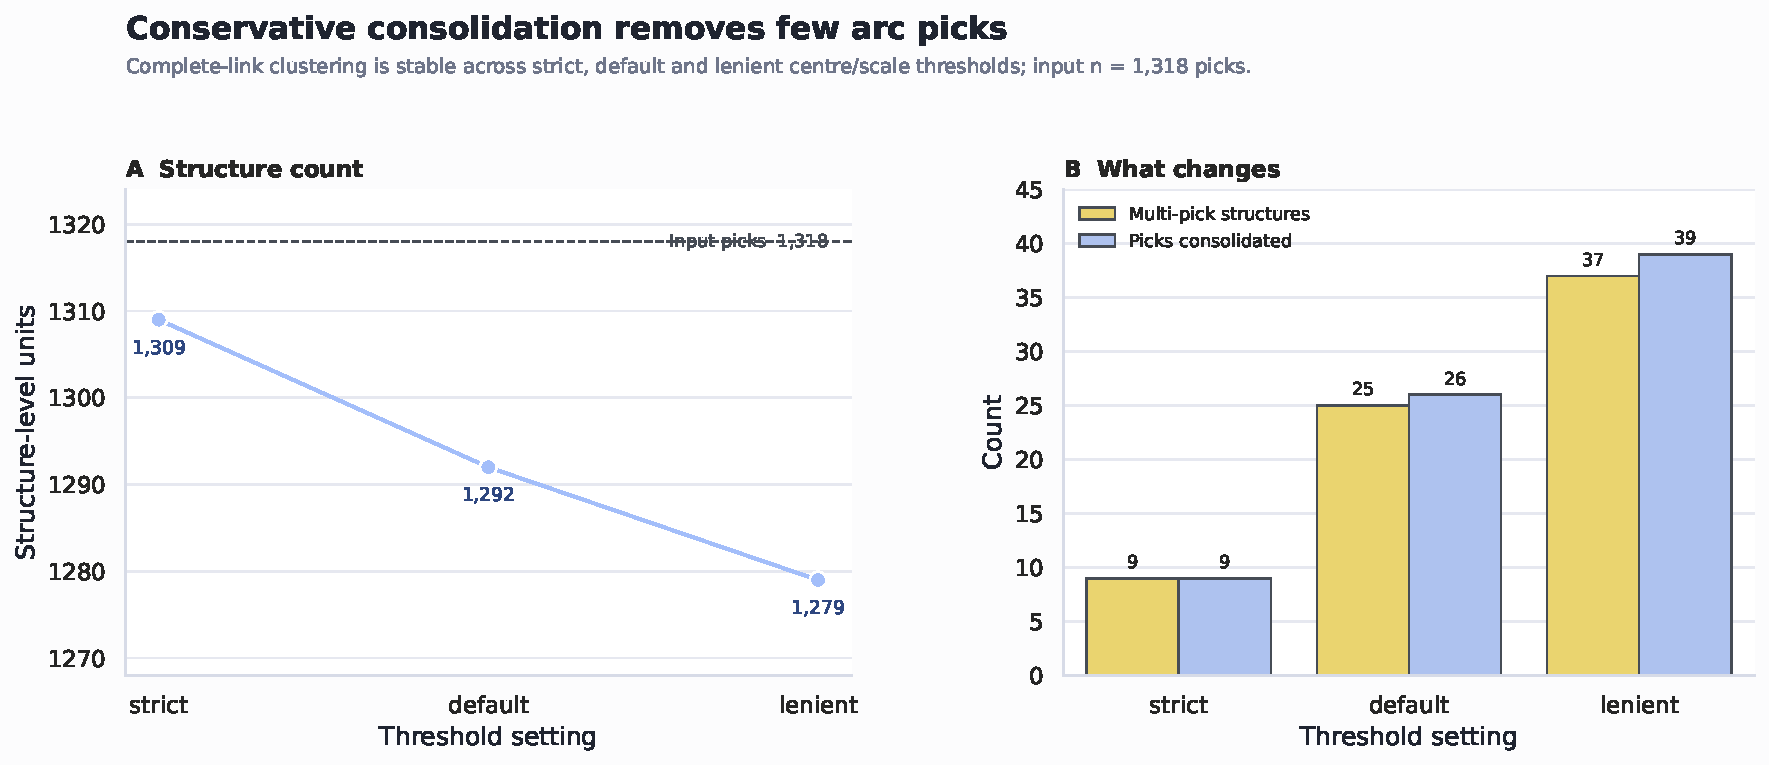
\includegraphics[width=0.96\textwidth]{figure_suite/fig_structure_consolidation.pdf}
  \caption{Sensitivity of structure-level consolidation to centre-separation and radius-ratio thresholds. The default complete-link rule removes only 26 of 1,318 picks, and plausible strict-to-lenient settings yield 1,309--1,279 units. Broad overlapping footprints are not automatically merged.}
  \label{fig:consolidation}
\end{figure}

The 32 Tier A/B structure-level cases have an active-fault intersection fraction of 0.156, compared with a matched-null mean of 0.165 ($p=0.639$). Their median log-transformed nearest-fault distance divided by radius is also not unusually small ($p=0.294$; Figure~\ref{fig:fault-nulls}). Thus the current highest-priority set is not detectably concentrated on mapped active faults after coarse geographic and scale matching. This is a useful negative control, but it does not exclude older inactive structures, unmapped faults or non-fault tectonic and igneous origins.

\begin{figure}[H]
  \centering
  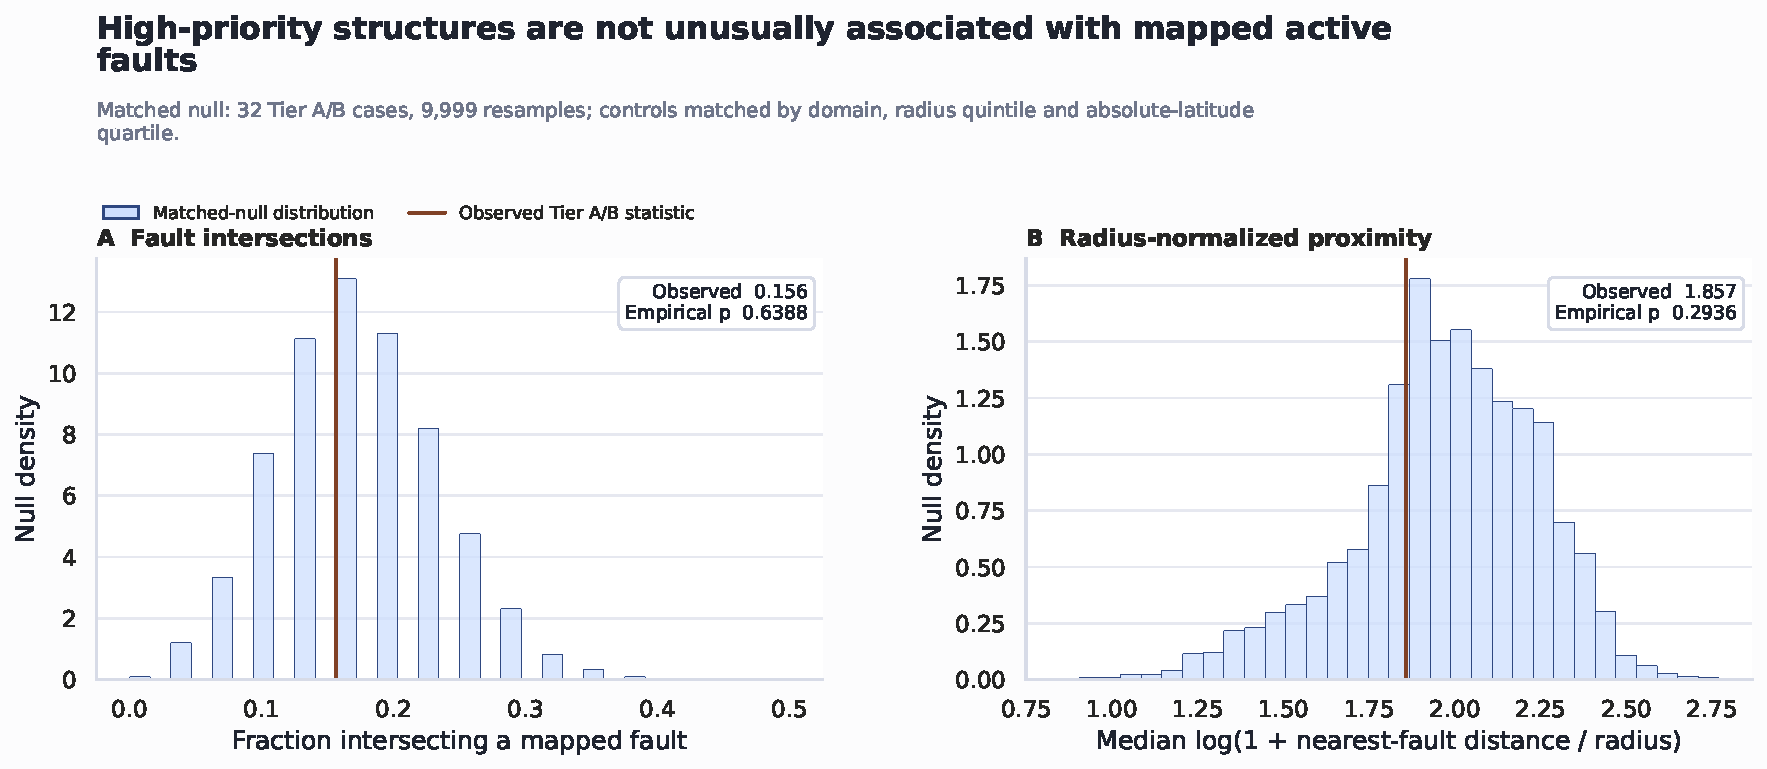
\includegraphics[width=0.98\textwidth]{figure_suite/fig_fault_matched_nulls.pdf}
  \caption{Matched-null distributions for mapped active-fault intersection and radius-normalized proximity. Orange lines show the observed Tier A/B statistics; controls are matched by land/ocean domain, radius quintile and absolute-latitude quartile. Neither statistic is significantly enriched in the impact-candidate direction.}
  \label{fig:fault-nulls}
\end{figure}

\subsection{Gravity-first shortlist, endogenic controls and preservation}
The gravity-first extension retains \InductiveShortlistN\ candidates with review scores from \InductiveScoreMin\ to \InductiveScoreMax\ (median \InductiveScoreMedian). The shortlist contains \InductiveLandN\ land and \InductiveOceanN\ ocean candidates spanning 18.3--648.0~km. All meet the strong-gravity rule by construction; only \InductiveMagneticSupportN\ have separately supporting magnetic percentiles and \InductiveMagneticDiscordantN\ are magnetically discordant. This reinforces the global null result: gravity is the main independent remote-sensing lead, while magnetics is heterogeneous rather than a required channel. Table~\ref{tab:gravity-shortlist} lists the first ten rows.

\begin{table}[H]
\centering
\caption{First ten gravity-first review candidates. Morph., G, M and Review are morphology, gravity-consensus, stratified magnetic and gravity-first review scores. Preservation is a rule-based acquisition context, not a genetic diagnosis.}
\label{tab:gravity-shortlist}
\scriptsize
\begin{tabular}{@{}lrlrrrrp{3.2cm}@{}}
\toprule
Candidate & Diameter (km) & Domain & Morph. & G & M & Review & Preservation\\
\midrule
\texttt{arc\_0371} & 39.9 & ocean & 0.815 & 1.000 & 1.000 & 0.917 & buried sedimentary \\
\texttt{arc\_0674} & 157.7 & land & 0.765 & 0.993 & 0.329 & 0.891 & eroded exposed \\
\texttt{arc\_0687} & 254.4 & land & 0.771 & 0.984 & 0.705 & 0.890 & eroded exposed \\
\texttt{arc\_1088} & 147.2 & land & 0.789 & 0.966 & 0.534 & 0.890 & buried sedimentary \\
\texttt{arc\_1105} & 361.1 & ocean & 0.759 & 0.994 & 0.447 & 0.887 & buried sedimentary \\
\texttt{arc\_0795} & 91.2 & land & 0.772 & 0.974 & 0.724 & 0.886 & buried sedimentary \\
\texttt{arc\_0437} & 182.3 & ocean & 0.785 & 0.985 & 0.537 & 0.883 & oceanic volcanic or margin confounded \\
\texttt{arc\_0697} & 49.0 & land & 0.753 & 0.969 & 0.906 & 0.875 & buried sedimentary \\
\texttt{arc\_0605} & 44.9 & land & 0.800 & 0.917 & 0.575 & 0.873 & eroded exposed \\
\texttt{arc\_0899} & 274.1 & land & 0.747 & 0.967 & 0.557 & 0.871 & buried sedimentary \\

\end{tabular}
\end{table}

Candidate \texttt{arc\_0371} ranks first with morphology 0.815, gravity consensus 1.000 and magnetic percentile 1.000. It is not a clean discovery case: its centre lies 118~km from Anton Dohrn and the two occupy the same North Atlantic regional family. Anton Dohrn itself remains in the shortlist, demonstrating that a coherent morphology--gravity signal can arise from a known volcanic structure. Nine shortlisted candidates have a mapped active-fault trace crossing the candidate disk, so even high gravity-first rank does not remove tectonic alternatives.

\begin{figure}[H]
  \centering
  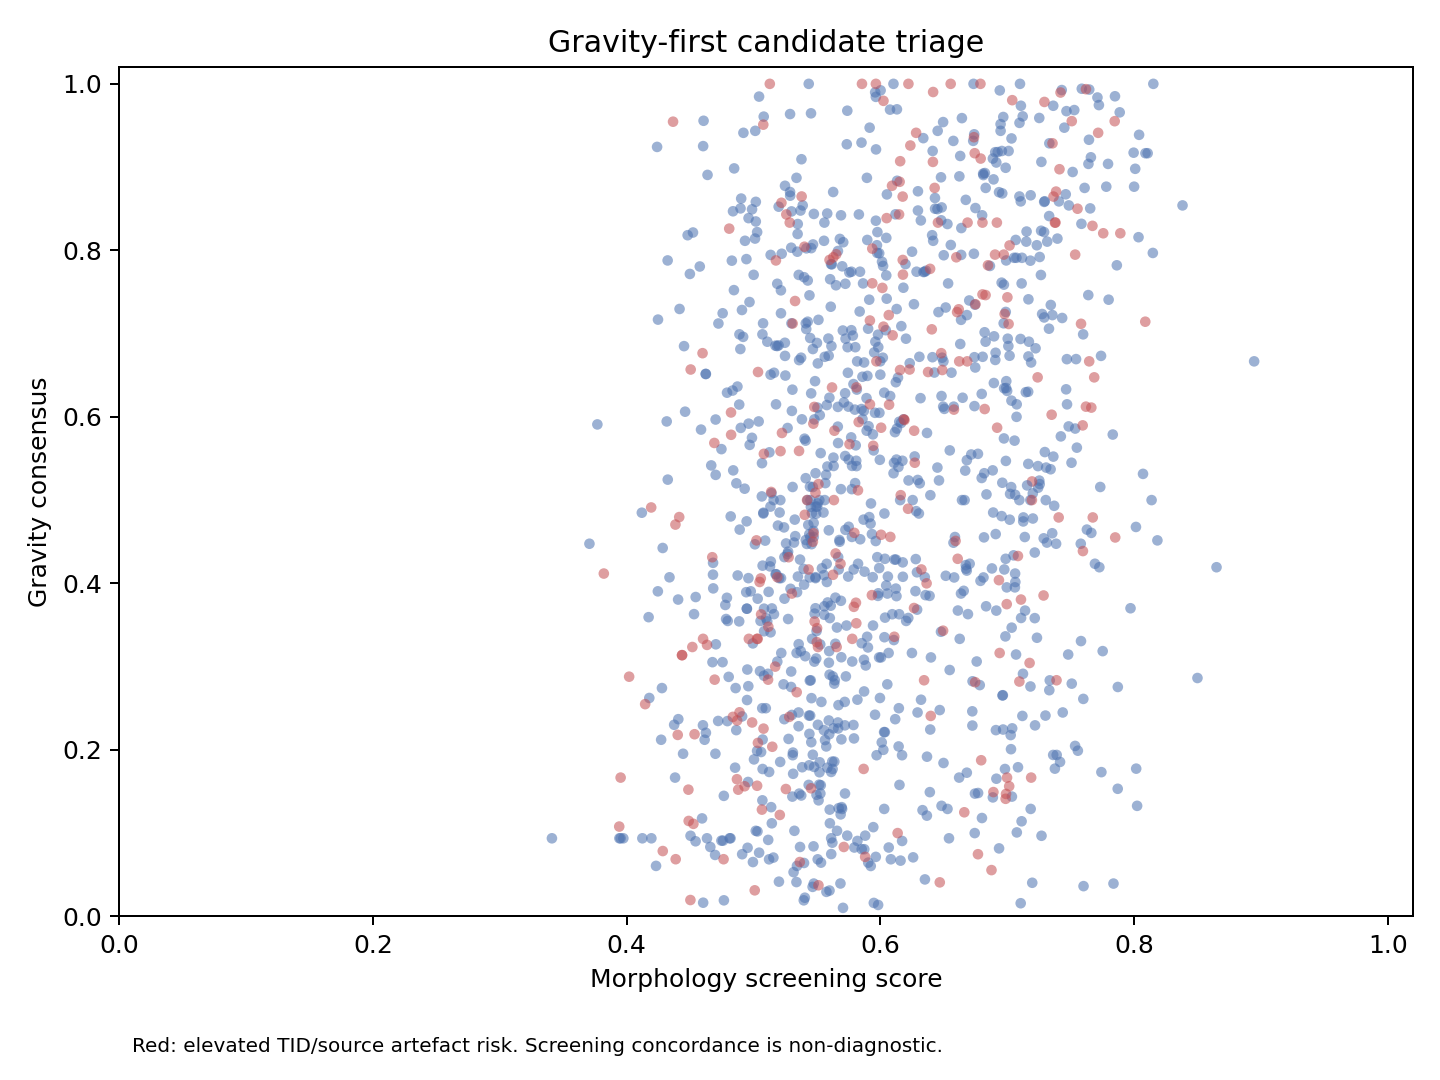
\includegraphics[width=0.92\textwidth]{outputs/figures/gravity_first_scatter.png}
  \caption{Morphology versus gravity consensus for the complete candidate inventory. Colour flags elevated GEBCO TID/source artefact risk. The upper-right population motivates review; it is not an impact-probability field.}
  \label{fig:gravity-first}
\end{figure}

The normalized control library contains \InductiveControlN\ endogenic comparators (Table~\ref{tab:control-library}). Of the 25 shortlist matches, only Anton Dohrn overlaps its corresponding candidate and triggers a control warning. None of the remaining shortlist centres is sufficiently near the five supplied African controls to trigger the proximity-gated similarity rule. This is preferable to the earlier size-only behaviour, but the small library cannot yet estimate false-positive rates by endogenic class.

\begin{table}[H]
\centering
\caption{Current endogenic negative-control library. Diameters are derived from supplied polygons except Anton Dohrn, which uses its fitted candidate geometry. Classes are comparator-oriented and do not replace detailed petrogenetic descriptions.}
\label{tab:control-library}
\small
\begin{tabular}{llrrr}
\toprule
Control & Comparator class & Latitude & Longitude & Diameter (km)\\
\midrule
Anton Dohrn Seamount & volcanic seamount & 57.432 & -11.120 & 60.2 \\
Brandberg/Messum & intrusive complex & -21.126 & 14.549 & 27.9 \\
Djebel Uweinat & ring complex & 21.915 & 24.907 & 25.3 \\
Jabal Arkanu & ring complex & 22.283 & 24.715 & 30.9 \\
Pilanesberg & ring complex & -25.250 & 27.078 & 26.1 \\
Richat & ring complex & 21.103 & -11.389 & 36.0 \\

\end{tabular}
\end{table}

\begin{figure}[H]
  \centering
  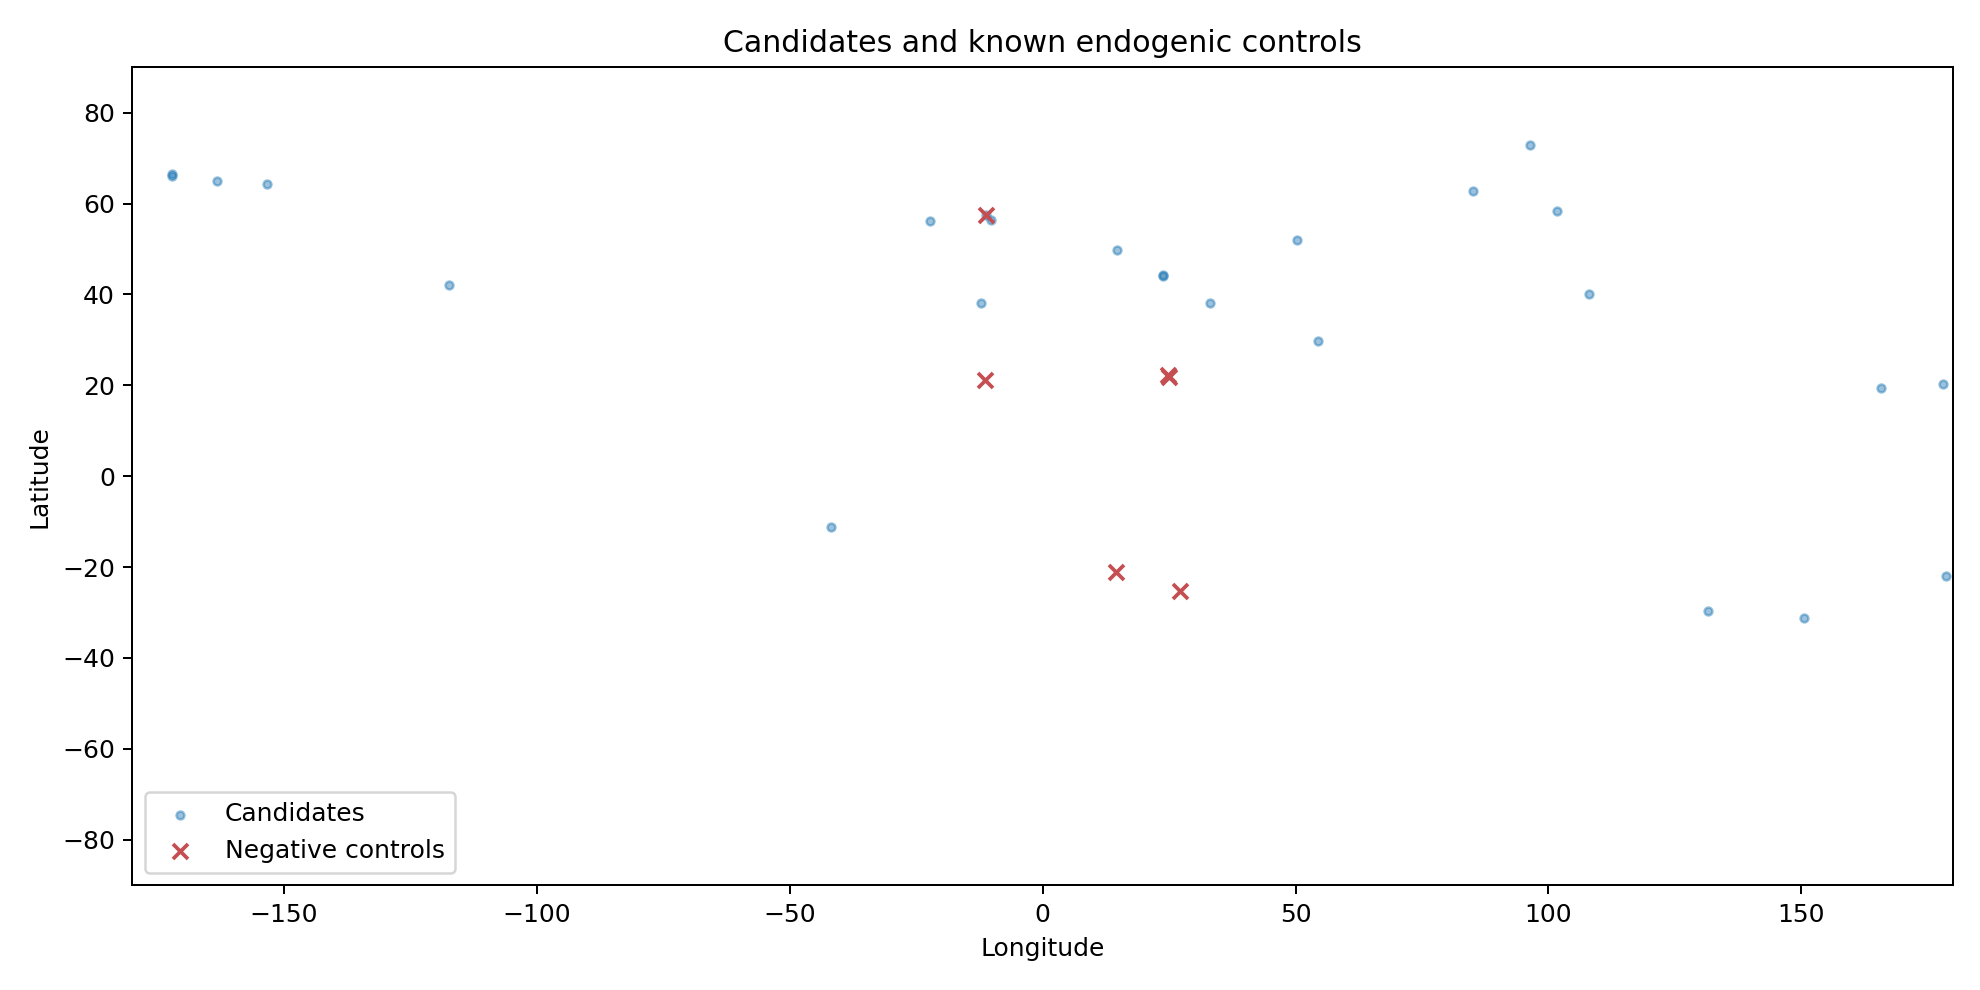
\includegraphics[width=0.96\textwidth]{outputs/figures/candidate_vs_controls_map.png}
  \caption{Locations of the 25 gravity-first candidates and six current endogenic controls. The library is deliberately shown as sparse and regionally uneven; distance from a plotted control is not evidence against an endogenic origin.}
  \label{fig:control-map}
\end{figure}

Preservation logic assigns 12 shortlist rows to buried sedimentary settings, eight to eroded/exposed settings, four to oceanic volcanic-or-margin-confounded settings and one to a fresh-or-shallow context (Table~\ref{tab:preservation}). All 25 receive gravity/seismic modelling priority under at least one rule, while the eight exposed cases provide the clearest near-term opportunities for mapped transects, archived sample review and petrography. Twenty regional-proximity families are present in the shortlist; eight candidates belong to multi-member clusters and two broad footprints overlap. These clusters should not be counted as independent hypotheses.

\begin{table}[H]
\centering
\caption{Rule-based preservation states for the 25 gravity-first candidates.}
\label{tab:preservation}
\begin{tabular}{lr}
\toprule
Predicted state & Candidates\\
\midrule
buried sedimentary & 12 \\
eroded exposed & 8 \\
oceanic volcanic or margin confounded & 4 \\
fresh or shallow & 1 \\

\end{tabular}
\end{table}

\subsection{Nested arcuate families and planetary geometry}
Complete-link testing identifies \InductiveRingFamilyN\ candidate nested families containing \InductiveRingMemberN\ geometries: \InductiveRingPairN\ pairs and \InductiveRingTripleN\ triples. Every final adjacent-radius ratio is at least 1.2. None of the 25 gravity-first shortlist rows belongs to one of these families, so nested geometry and gravity-first concordance currently define separate follow-up sets rather than mutually reinforcing evidence. The two three-member cases are \texttt{arc\_1241}/\texttt{arc\_1242}/\texttt{arc\_0419} (diameters 866--1,847~km) and \texttt{arc\_0957}/\texttt{arc\_0958}/\texttt{arc\_0959} (98--185~km).

\begin{figure}[H]
  \centering
  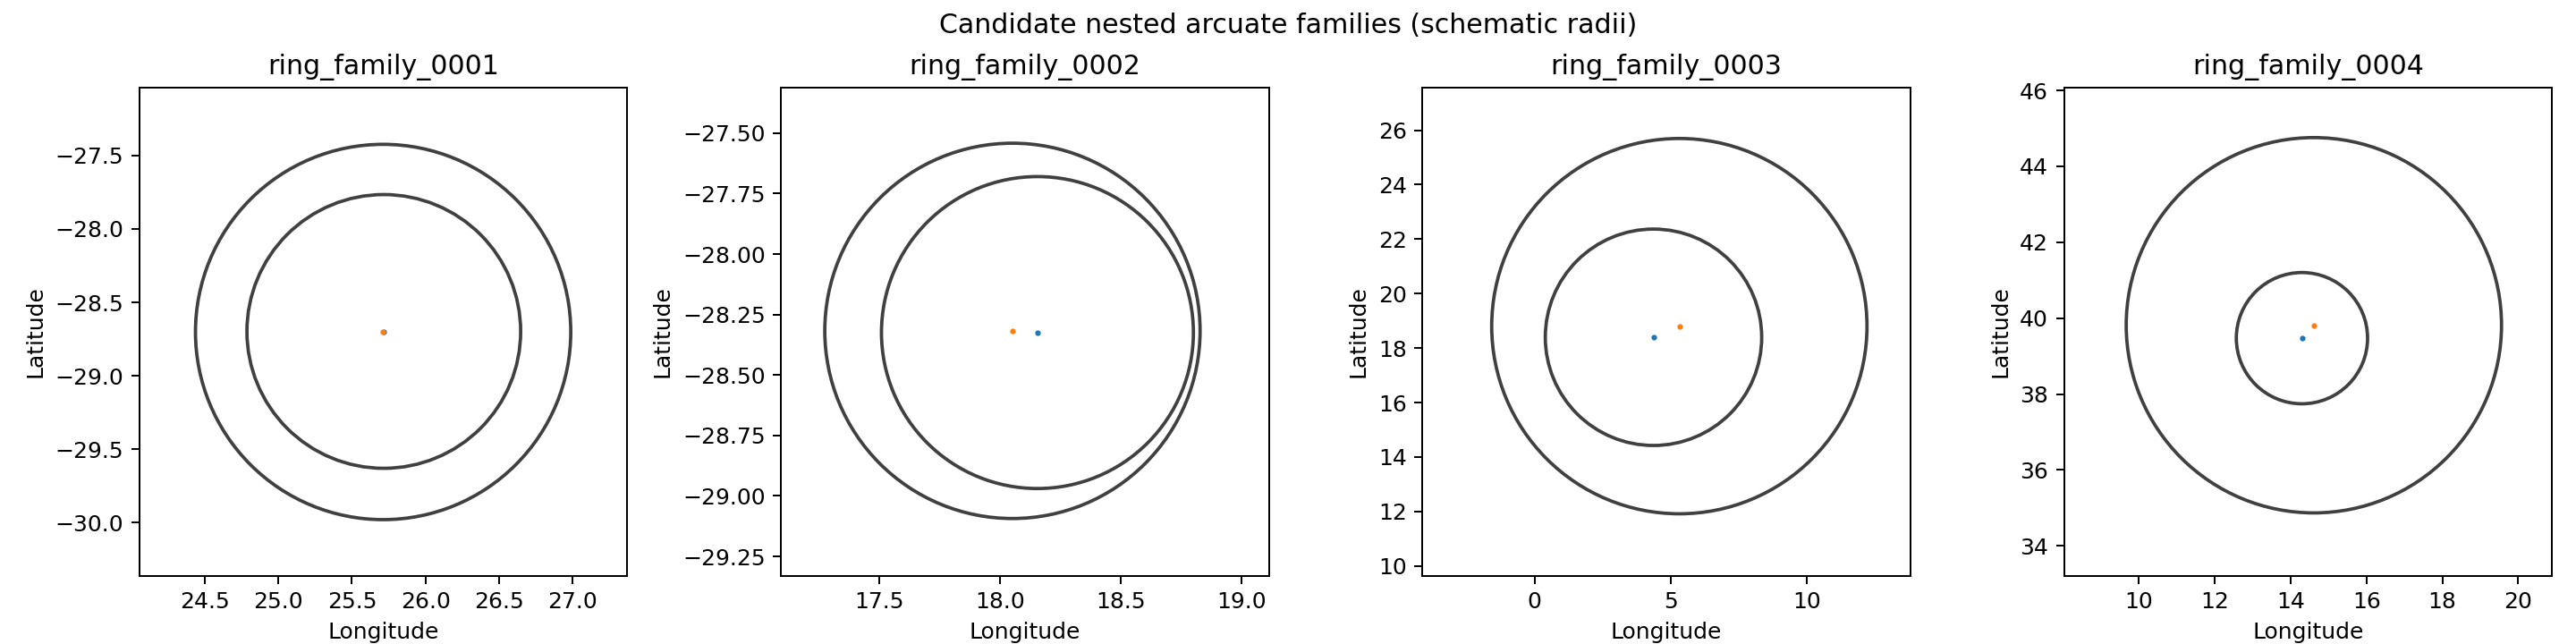
\includegraphics[width=0.98\textwidth]{outputs/figures/ring_family_examples.png}
  \caption{Schematic examples of complete-link candidate nested arcuate families. Circles show fitted centres and radii; they are geometric screening constructs and require geological discrimination.}
  \label{fig:ring-families}
\end{figure}

The median adjacent-ring ratio is 1.409 for terrestrial candidate families, 1.427 for the 11 published lunar multiring basins and 1.403 for the three historical Martian examples (Table~\ref{tab:planetary-comparison}). Their interquartile ranges overlap. This is a useful calibration of geometric plausibility but not an origin test: the terrestrial search explicitly truncates ratios below 1.2, the lunar table preserves mixed confidence levels, and the Martian subset is small and historical. Terrestrial outer diameters range from 23 to 2,226~km, overlapping the lunar 571--1,321~km scale and reaching the lower part of the Martian 1,900--5,500~km scale.

\begin{table}[H]
\centering
\caption{Geometric comparison of terrestrial candidate families and published planetary basin subsets. Ratio IQR is the 25th--75th percentile of sorted adjacent-ring ratios.}
\label{tab:planetary-comparison}
\scriptsize
\begin{tabular}{@{}p{3.2cm}rrrrr@{}}
\toprule
Set & Families/basins & Ratios & Median ratio & Ratio IQR & Diameter range (km)\\
\midrule
Terrestrial candidate families & 26 & 28 & 1.409 & 1.362--1.756 & 23--2226 \\
Published lunar multiring basins & 11 & 30 & 1.427 & 1.348--1.599 & 571--1321 \\
Historical Martian subset & 3 & 14 & 1.403 & 1.276--1.426 & 1900--5500 \\

\end{tabular}
\end{table}

\begin{figure}[H]
  \centering
  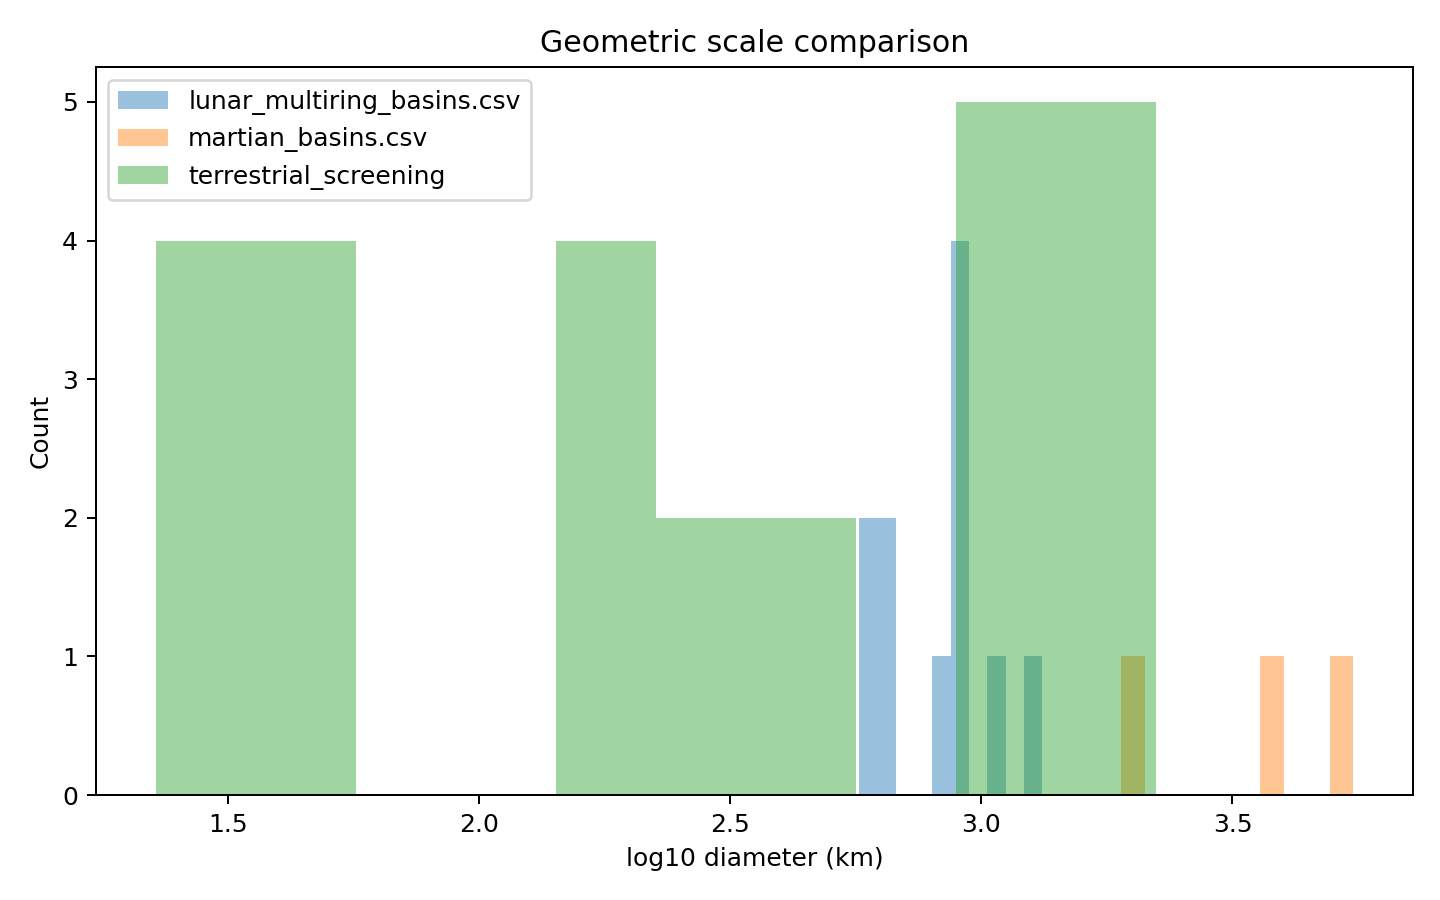
\includegraphics[width=0.88\textwidth]{outputs/figures/planetary_size_comparison.png}
  \caption{Diameter distributions for terrestrial candidate families and the lunar and Martian comparison subsets. Similar scale is geometric context only and cannot transfer a planetary impact classification to a terrestrial feature.}
  \label{fig:planetary-size}
\end{figure}

\section{Discussion}
The updated data do not sustain the original quantitative argument for widespread distal shock boundaries. The current arc inventory is larger than the one described previously, both impact catalogues require explicit analytical grains, and the old log--log slopes were method-dependent. Repair changes the fitted multiplier from 5.53 to 9.10 and removes the earlier significant residual shape difference. This keeps size scaling open as a statistical hypothesis, but provides no physical validation of a universal conversion. French's crater-formation model sharpens that distinction: shock pressure attenuates rapidly, whereas large rings are modification-stage structures generated by uplift, collapse and faulting \cite[pp.~18--29]{French1998}. Well-studied basins further show that ring dimensions depend on which structural element is measured, impact energy, gravity, target rheology, thermal state and post-impact modification \cite{French1998,Potter2013,Gulick2013}. A universal multiplier would erase precisely the geological variation that needs explanation.

The longitude-rotation result is nevertheless worth following up. It shows that the EID-matched subset is nearer the arc inventory than expected after breaking longitudinal alignment while preserving latitude and catalogue configuration. The failure of the confidence-label null is the crucial control: proposed entries are similarly close. This can arise from common geographic sampling, deliberate compilation of visually circular features, shared source catalogues, or genuine geological clustering. With current provenance it cannot be attributed specifically to impact.

The gravity result strengthens the case for cross-layer follow-up but not for impact. Gravity and bathymetry are physically coupled in volcanic edifices, sedimentary basins, continental margins and other endogenic structures. The Bangui anomaly provides a particularly relevant African precedent: a striking magnetic anomaly associated with broad gravity and ring-like structure motivated an impact model \cite{Girdler1992}, yet regional reprocessing linked it to a larger Bangui--Atlantic feature and left the genetic relation equivocal \cite{ReimoldKoeberl2014}. Richat provides the complementary morphology-first warning: its exceptional bull's-eye form was historically proposed as impact-related, but field relationships, igneous features, karst-collapse breccia and the absence of accepted diagnostic shock evidence support an endogenic and erosional interpretation \cite{ReimoldKoeberl2014}. Anton Dohrn Seamount (candidate \texttt{arc\_0370}) falls in the strongest operational tier and is therefore a mandatory negative control: the method correctly recognizes a coherent circular topographic--gravity structure while offering no basis for assigning its cause.

The expanded control library makes that caution operational rather than rhetorical. Richat, Pilanesberg, Jabal Arkanu, Djebel Uweinat and Brandberg/Messum now enter the same spatial-matching workflow as Anton Dohrn. Only Anton overlaps a shortlisted candidate, so the current run does not show that the other controls explain the shortlist. Nor could it: six controls are too few and too geographically concentrated to estimate class-conditional false-positive rates. The immediate value is procedural. New calderas, ring complexes, diapirs, salt structures and sedimentary basins can be appended without changing the analysis code, and distant structures of similar diameter no longer generate spurious warnings.

The planetary comparison provides a second calibration with a different limitation. Terrestrial candidate ratios occupy the same broad range as published lunar and historical Martian rings, which shows that the fitted nesting is not geometrically absurd. Yet the terrestrial distribution is conditioned on the 1.2 search threshold and visual source inventory, while planetary basins were classified from independent topography, gravity and geological mapping \cite{Neumann2015,PikeSpudis1987}. The overlap therefore cannot validate impact origin or a universal spacing law. Its useful role is candidate-specific: a proposed nested family can now be compared with explicit ring sequences and confidence labels rather than a single global 9.10 multiplier.

Within the structural-inheritance hypothesis, a present volcanic, tectonic or hydrological expression does not by itself falsify an older impact contribution: later processes are the proposed mechanism by which buried structural memory becomes visible. The converse is equally important. Because those same endogenic processes generate arcuate morphology and gravity anomalies without impact, their presence is not evidence of inheritance. Demonstration requires temporal and spatial ordering: an older concentric damage architecture must be shown to pre-date and localize younger faulting, magmatism, fluid flow or erosion, and the relationship must outperform matched endogenic controls.

The next gravity phase should therefore move from global ring-score screening to candidate-centred anomaly morphology, wavelength and amplitude modelling, including forward density models and blinded comparisons with confirmed impacts and endogenic controls. Candidate-specific electrical-resistivity modelling at the proposed Sirente structure illustrates how geophysical forward models can test predicted shallow architecture and alternatives while remaining supportive rather than confirmatory \cite{Torrese2022}. Neither the active-fault intersection nor proximity null is significant, so active faulting does not explain the top tiers at this resolution; equally, the incomplete, neotectonic GEM layer cannot rule out ancient tectonic inheritance. The non-significant magnetic result further argues against treating multi-layer appearance as automatic corroboration. Lithology, geological age, inactive structures and plausible endogenic classes remain necessary controls.

Morphology is additionally non-independent here. The arcs were selected visually from GEBCO and then scored against GEBCO, and most features are near-perfect sampled circles, so their circularity largely records observation and data construction rather than out-of-sample geological fit. The current nulls preserve latitude, domain and broad scale but do not reproduce interpreter effort, regional search intensity, spatial autocorrelation or detailed tectonic setting. French explicitly warns that there is no morphological or geophysical criterion that unambiguously separates impact structures from other circular geological features \cite[pp.~97--99]{French1998}. Confirmation must therefore move outside these geometry files. At minimum, a candidate needs mapped stratigraphic disruption and geophysical consistency; verification requires accepted shock-metamorphic, meteoritic or geochemical evidence \cite{French1998,FrenchKoeberl2010,Osinski2022}.

The distinction between distal deformation and distal ejecta also changes the most productive search strategy. If an ancient impact basin has lost its upper structural levels, the surviving evidence may not be a giant circular fracture. It may instead consist of a partial central uplift, discontinuous breccias or pseudotachylites, shocked mineral grains in isolated outcrops, buried gravity/seismic structure, or stratigraphically preserved ejecta outside the crater \cite[pp.~28--30, 78, 97--103]{French1998}. Candidate assessment should therefore combine geometry with predicted preservation state rather than require a complete ring.

\section{Recommended additions and improvements}
The following changes would make the project substantially more discriminating.

\begin{enumerate}
  \item \textbf{Add provenance and confidence fields.} For every arc, record the source map or imagery, interpreter, acquisition date, geological unit, feature class, original (unbuffered) trace and reason for inclusion. Separate observed lineaments from circles generated during processing.
  \item \textbf{Expand and balance the negative-control library.} The current six controls establish the workflow but not a false-positive rate. Add volcanic calderas, seamounts, ring complexes, diapirs, salt structures, sedimentary basins, intrusive complexes and tectonic arcs across land/ocean domains and diameter strata. A classifier or enrichment test is informative only if impact candidates outperform plausible endogenic alternatives selected with comparable search effort.
  \item \textbf{Model the observation process.} Restrict comparisons to regions with comparable exposure and imagery, or include land/ocean mask, crustal age, sediment cover, tectonic setting and survey effort. Longitude rotation alone cannot represent these biases.
  \item \textbf{Validate catalogue status.} Reconcile every local EID-match flag with a dated authoritative snapshot and preserve persistent identifiers and citations. Keep confirmed, probable, proposed and rejected structures in separate tables.
  \item \textbf{Quantify geometric uncertainty.} Fit circles or small circles to original traces, report angular coverage and radial residuals, and propagate centre/diameter uncertainty into the spatial and size tests. Very short arcs can admit many possible circles.
  \item \textbf{Test centre and scale jointly.} For pre-registered high-priority candidates, compare concentricity and ring ratios with structure-specific excavation/modification models rather than a global multiplier. Nested rings, gravity/magnetic anomalies, target geology and expected preservation state should agree spatially. Shock-pressure decay should be modelled separately from modification-stage ring formation.
  \item \textbf{Test structural inheritance chronologically.} For selected candidates, determine whether deep concentric faults, permeability or density architecture predates and localizes younger tectonism, magmatism, fluid flow or erosion. Compare rates of later reactivation around confirmed ancient impacts with tectonic, volcanic and basin controls matched by crustal age, lithology and setting.
  \item \textbf{Pursue candidate-scale gravity modelling.} For Tier A/B structures and matched endogenic controls, extract higher-resolution gravity where available, separate regional and residual fields, test concentric anomaly wavelengths and amplitudes, and fit alternative density models for brecciation, melt, uplift, basin fill, volcanism and intrusion. Pre-register discriminating predictions before interpreting individual targets.
  \item \textbf{Apply French's detection-to-verification funnel.} Screen by morphology; seek independent gravity, magnetic or seismic support; map predicted uplift, faulting and brecciation; then target outcrop, archived core or new drilling for material evidence \cite[pp.~97--100]{French1998}.
  \item \textbf{Prioritize field falsification.} Rank candidates by independent geophysical support and accessible outcrop, then search blind petrographic samples for well-developed shatter cones, crystallographically controlled planar deformation features, diaplectic glass, high-pressure polymorphs or projectile geochemistry. Negative results should remain in the dataset to prevent repeated rediscovery.
\end{enumerate}

\section{Conclusions}
The revised analysis converts an apparent visual correspondence into a falsifiable screening study. The current data contain 1,318 arc geometries, conservatively consolidated to 1,292 structure-level units, 80 named African structures and 249 repaired, deduplicated global catalogue entries. A statistically fitted diameter multiplier is 9.10, and the corrected test does not reject distributional compatibility after scaling ($p=0.145$); this leaves the size-scaling hypothesis open without establishing a universal physical law. EID-matched centres show non-random proximity under longitude rotation, yet no enrichment over proposed catalogue entries under a stronger within-catalogue control. Gravity is independently concordant with the morphology inventory, but magnetics are not, a mapped-active-fault control is non-significant, and a volcanic negative control ranks strongly. The inductive extension turns these findings into a 25-candidate gravity-first review queue, preservation-dependent tests, six explicit endogenic controls, 26 complete-link nested families and a confidence-preserving planetary geometry comparison. None of these additions supplies diagnostic impact evidence: Anton Dohrn remains highly ranked, no top-25 candidate is also a nested-family member, and planetary ratio overlap is conditioned by selection. Read through French's recognition framework, the defensible conclusion remains limited: the inventories share spatial and gravity structure, but they do not demonstrate that the arcs are impact-generated rings, shock-pressure boundaries or distal ejecta. Testing the broader structural-inheritance hypothesis requires chronology and deep structural continuity, while confirmation of individual impacts still depends on preservation-aware geology, geophysics and diagnostic material evidence rather than additional visual overlap.

\section*{Reproducibility}
Catalogue statistics, tables and figures are generated by \path{analysis.py} using the arc inventory, the African source file and \path{catalog_repair/astroblemes_analysis.geojson}. Catalogue repair is generated by \path{repair_astrobleme_catalog.py}; its dated source snapshots, row-level audit and immutable original are retained under \path{catalog_repair}. Geophysical evidence is generated by \path{enrich_arc_ranking.py}. Null rows and summaries are generated by \path{run_geophysical_nulls.py} and \path{summarize_geophysical_nulls.py}; operational tiers are generated separately by \path{build_geophysical_shortlist.py}. Structure consolidation and GEM controls are generated by \path{consolidate_structures_and_faults.py}, with outputs under \path{structure_output} and the source fault snapshot under \path{geology_sources}. The inductive extension is generated by \path{scripts/run_inductive_pipeline.py}; planetary tables by \path{scripts/build_planetary_catalogues.py}; and manuscript table fragments by \path{scripts/build_inductive_manuscript_assets.py}. Endogenic controls are read from \path{data/controls.geojson} and the built-in Anton Dohrn record. Seeds are 20260619 for catalogue tests, 20260621 for geophysical tests, 954 for the matched fault null and 42 for deterministic inductive configuration. Machine-readable outputs and figure pairs are consumed directly by this document. A 1,318-feature review layer with scores, evidence fields and blank manual-capture fields is provided at \path{study_results_geojson/arcuate_geometries_study_results.geojson}; its field definitions are preserved in the adjacent schema JSON.

\section*{Supplementary spatial context}
Figure~\ref{fig:structure-map} shows the geographic distribution of consolidated units, high-priority tiers, multi-pick units and the GEM fault layer. It is presented as context rather than an inferential map because GEM coverage is uneven and especially incomplete offshore.

\begin{figure}[H]
  \centering
  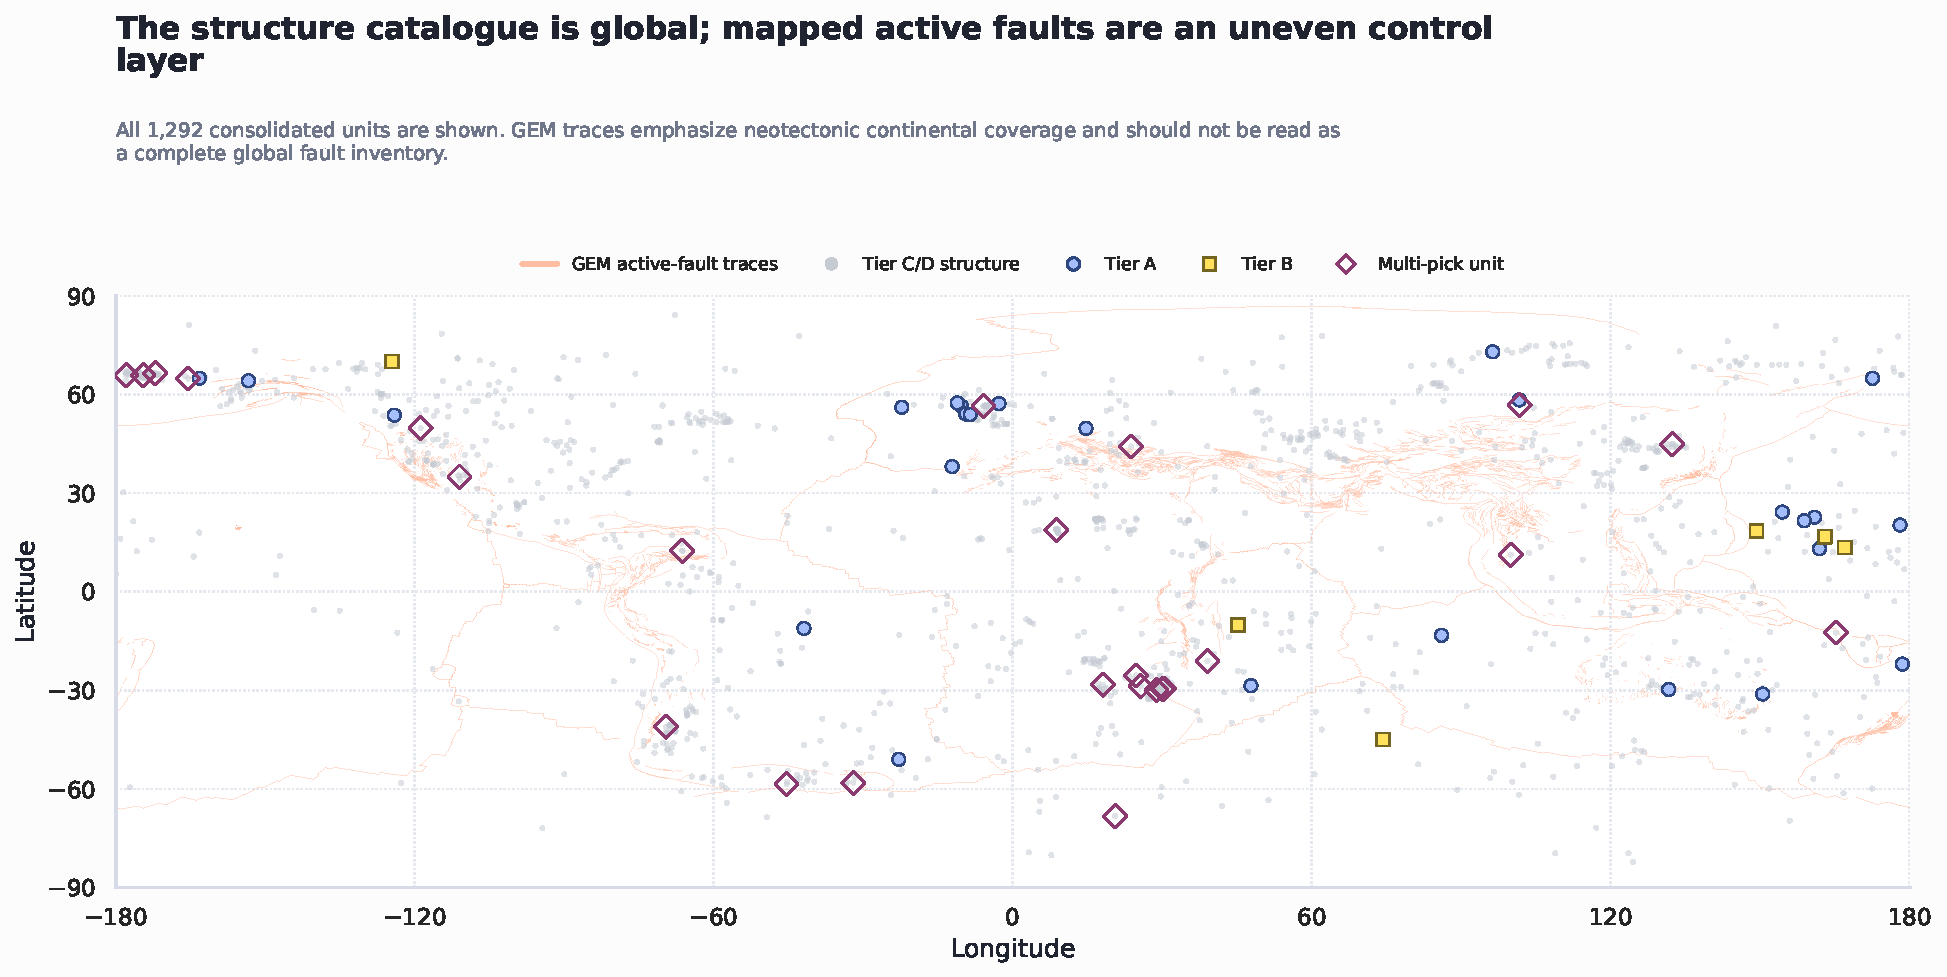
\includegraphics[width=0.98\textwidth]{figure_suite/fig_structure_global_map.pdf}
  \caption{Global distribution of the 1,292 consolidated structure-level units, operational Tier A/B cases, multi-pick units and harmonized GEM active-fault traces. The visible concentration of fault traces partly reflects database coverage and must not be interpreted as a uniform global absence/presence test.}
  \label{fig:structure-map}
\end{figure}

\clearpage
\appendix
\section{Additional visual-identification contexts}
Figures~\ref{fig:drake-context-satellite} and \ref{fig:drake-context-colour} show two further visual contexts used when reviewing the Drake Passage region. They contain the same kind of interpretive candidate overlays as Figure~\ref{fig:drake-identification}, but use different background treatments to expose complementary aspects of coastlines, regional relief and seafloor fabric. These are examples of the compilation environment rather than independent analytical layers or validation images.

\begin{figure}[H]
  \centering
  \includegraphics[width=0.98\textwidth]{drake1.png}
  \caption{Drake Passage candidate geometries over a natural-colour land and shaded-bathymetry context. This treatment supported simultaneous inspection of coastlines, islands, continental morphology and seafloor fabric. Gold circles are interpretive candidate overlays and are not geological confirmations.}
  \label{fig:drake-context-satellite}
\end{figure}

\begin{figure}[H]
  \centering
  \includegraphics[width=0.98\textwidth]{drake2.png}
  \caption{The Drake Passage overlays viewed with a colour-stretched elevation and bathymetry treatment. The enhanced relief provided a complementary visual context for recognizing partial arcs across strong regional gradients; apparent circularity in this view remains non-unique and was used only for candidate screening.}
  \label{fig:drake-context-colour}
\end{figure}

\clearpage
\section{Contrasting ranked terrain-diagnostic examples}
Figures~\ref{fig:rank-0593}--\ref{fig:rank-0284} contrast one high cross-layer review case, a known volcanic negative control and three high morphology-ranked but gravity-weak cases. Each panel presents raw GEBCO elevation, Gaussian-detrended terrain with the fitted candidate circle, and the magnitude of radial-gradient evidence within the normalized search annulus. The black contour marks the fitted radius ($\rho=1$); cyan contours mark $\rho=0.85$ and $1.15$.

These examples illustrate both the utility and limitation of the two-stage ranking. Candidate \texttt{arc\_0593} is the highest cross-layer review case, whereas Anton Dohrn is a Tier A volcanic control that proves the same rule can elevate an endogenic structure. Candidates \texttt{arc\_0306}, \texttt{arc\_0992} and \texttt{arc\_0284} rank highly by morphology but remain Tier C because they lack strong cross-layer gravity support (Table~\ref{tab:ranked-examples}). None is an impact confirmation.

\begin{table}[H]
\centering
\caption{Summary of the illustrated morphology-ranked candidates. Gravity and magnetic values are percentiles within the operational domain/scale comparisons; higher values indicate stronger relative screening evidence, not impact probability.}
\label{tab:ranked-examples}
\small
\resizebox{\textwidth}{!}{%
\begin{tabular}{llrrrrrr}
\toprule
Candidate & Role & Morph. rank & Review rank & Score & Diameter (km) & Gravity pct. & Magnetic pct.\\
\midrule
\texttt{arc\_0593} & Tier A & 4 & 1 & 0.838 & 77.7 & 0.854 & 0.699\\
\texttt{arc\_0370} & Tier A control & 9 & 4 & 0.811 & 60.2 & 0.917 & 0.583\\
\texttt{arc\_0306} & Tier C & 2 & 34 & 0.865 & 28.6 & 0.419 & 0.589\\
\texttt{arc\_0992} & Tier C & 3 & 35 & 0.850 & 20.0 & 0.286 & 0.177\\
\texttt{arc\_0284} & Tier C & 21 & 43 & 0.797 & 32.6 & 0.370 & 0.252\\
\bottomrule
\end{tabular}
}
\end{table}

\clearpage
Table~\ref{tab:ranking-contrasts} extends the comparison to candidates that are scientifically informative because evidence channels disagree, a regional or tectonic confound is present, or the candidate lies near a scale limit. These rows are not an additional priority tier. They are diagnostic cases for testing why the ranking succeeds or fails.

\begin{table}[H]
\centering
\caption{Notable discordant, clustered and confounded ranking examples. G and M are gravity-consensus and stratified magnetic percentiles; TID is the GEBCO source-transition artefact-risk score. Values are screening diagnostics, not impact probabilities.}
\label{tab:ranking-contrasts}
\scriptsize
\resizebox{\textwidth}{!}{%
\begin{tabular}{lrrrrrp{0.37\textwidth}}
\toprule
Candidate & Diameter (km) & Morph. score & G pct. & M pct. & TID risk & Interpretive value\\
\midrule
\texttt{arc\_0371} & 39.9 & 0.815 & 1.000 & 1.000 & 0.000 & Strongest all-channel concordance, but only 118~km from the Anton Dohrn volcanic control; test as part of a North Atlantic regional family.\\
\texttt{arc\_0373} & 67.2 & 0.895 & 0.667 & 0.917 & 0.003 & Highest morphology score yet Tier C because gravity support is only moderate; isolates morphology--gravity disagreement.\\
\texttt{arc\_0650} & 755.0 & 0.762 & 0.994 & 0.987 & 0.368 & Near-maximal gravity and magnetic support but elevated TID risk, three consolidated picks and a mapped active-fault intersection.\\
\texttt{arc\_0795} & 91.2 & 0.772 & 0.974 & 0.724 & 0.000 & Tier A land case with a mapped fault crossing the candidate disk and only 2.5~km from the centre; strong tectonic-confound test.\\
\texttt{arc\_0522} & 285.4 & 0.804 & 0.816 & 0.132 & 0.000 & Strong gravity but very weak magnetic percentile, plus a mapped fault intersection; useful for competing density and tectonic models.\\
\texttt{arc\_0752} & 373.2 & 0.800 & 0.876 & 0.965 & 0.219 & Large oceanic Tier A case paired regionally with \texttt{arc\_0753}; their broad footprints overlap.\\
\texttt{arc\_0753} & 519.5 & 0.780 & 0.904 & 0.962 & 0.209 & Centre lies 243~km from \texttt{arc\_0752}; the pair may represent one regional fabric rather than independent structures.\\
\texttt{arc\_0341} & 17.4 & 0.815 & 0.797 & 0.672 & 0.000 & Smallest Tier A case and a useful calibration check immediately above the severe sub-10-km resolution regime.\\
\texttt{arc\_0886} & 648.0 & 0.710 & 1.000 & 0.452 & 0.158 & Perfect gravity percentile but Tier D, with substantial boundary coincidence and a mapped fault crossing the disk; gravity-alone rejection control.\\
\bottomrule
\end{tabular}
}
\end{table}

Three follow-up groups emerge from this comparison. The North Atlantic cases should be reviewed jointly with Anton Dohrn rather than as independent discoveries. Candidates \texttt{arc\_0650}, \texttt{arc\_0795}, \texttt{arc\_0522} and \texttt{arc\_0886} are suited to blinded tectonic, volcanic and density-model alternatives. The \texttt{arc\_0752}/\texttt{arc\_0753} pair and the 755-km \texttt{arc\_0650} should be analysed in the large-structure scale regime before candidate-specific impact hypotheses are entertained.

\begin{figure}[H]
  \centering
  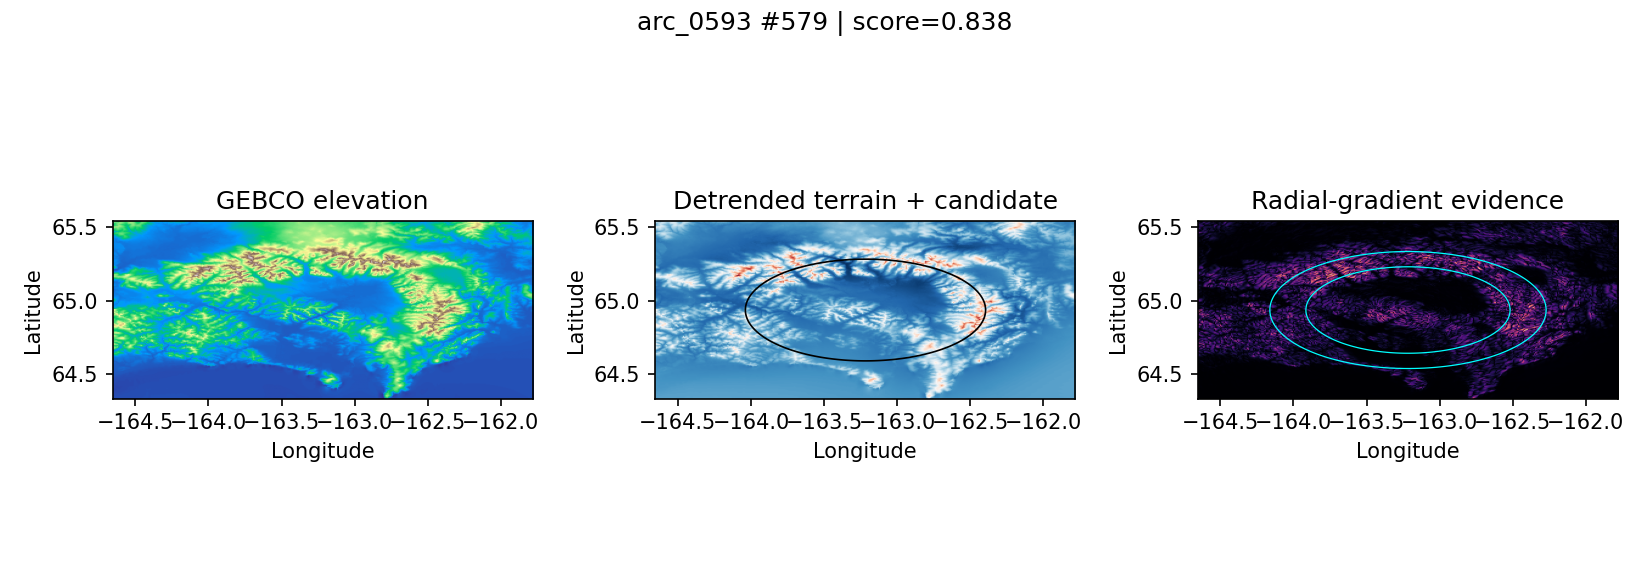
\includegraphics[width=0.98\textwidth]{ranking_output/diagnostics/arc_0593.png}
  \caption{Candidate \texttt{arc\_0593} at $64.935^{\circ}$N, $163.216^{\circ}$W. Its 77.7-km fitted geometry has morphology score 0.838 (rank 4) and gravity-consensus percentile 0.854, placing it first in the cross-layer review queue. The terrain follows a complex mountain-and-basin system, so the ranking motivates geological discrimination rather than an impact interpretation.}
  \label{fig:rank-0593}
\end{figure}

\begin{figure}[H]
  \centering
  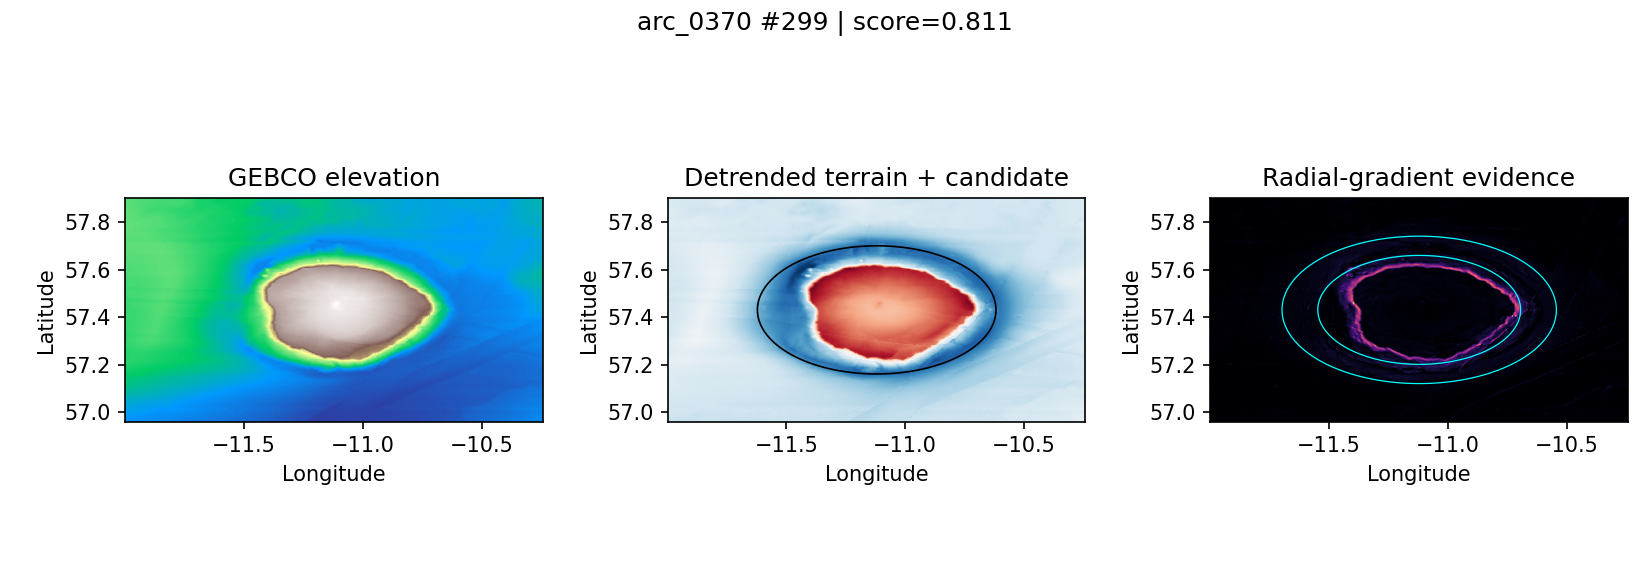
\includegraphics[width=0.98\textwidth]{ranking_output/diagnostics/arc_0370.png}
  \caption{Anton Dohrn Seamount, candidate \texttt{arc\_0370}, at $57.432^{\circ}$N, $11.120^{\circ}$W. Its 60.2-km fitted geometry has morphology score 0.811 and gravity-consensus percentile 0.917, placing it in Tier A despite its known volcanic origin. It is the principal negative control for interpreting cross-layer circularity.}
  \label{fig:rank-0370}
\end{figure}

\begin{figure}[H]
  \centering
  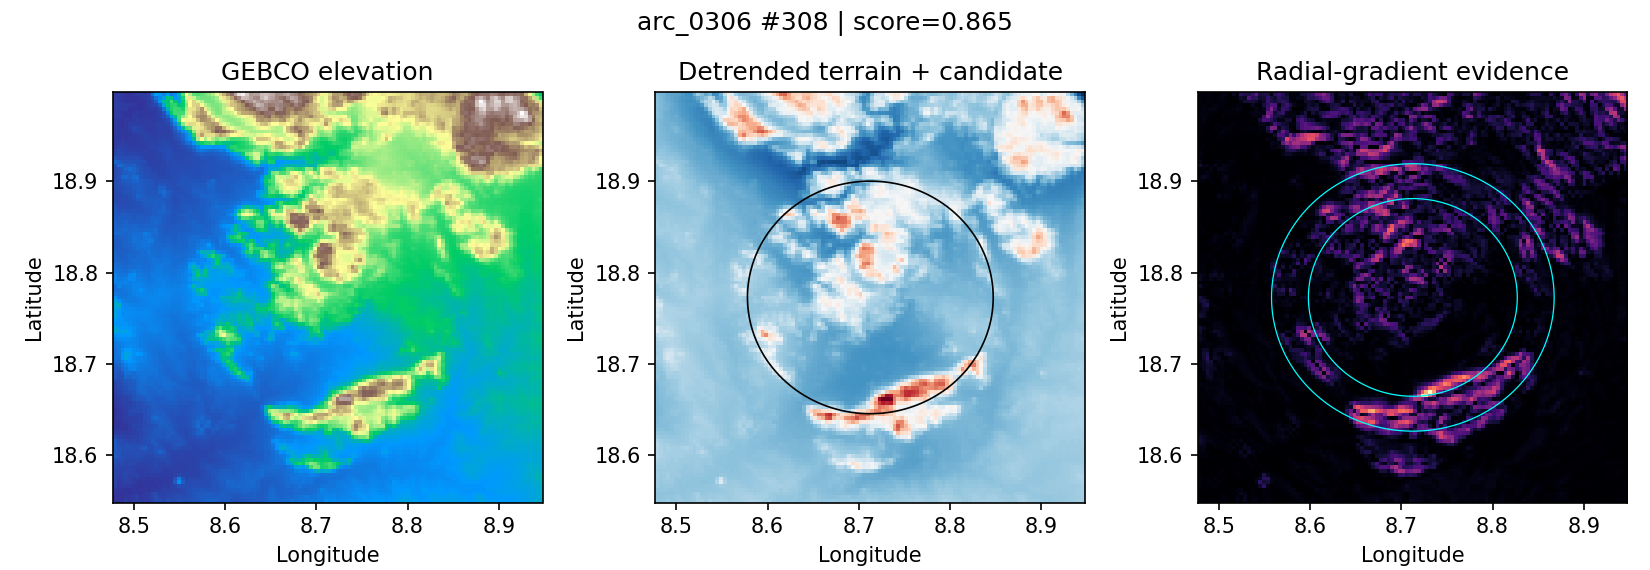
\includegraphics[width=0.98\textwidth]{ranking_output/diagnostics/arc_0306.png}
  \caption{Candidate \texttt{arc\_0306} at $18.773^{\circ}$N, $8.713^{\circ}$E. Its 28.6-km fitted geometry has morphology follow-up score 0.865 (rank 2), with a strong partial southern annular gradient. Its gravity-consensus percentile is 0.419, so it remains Tier C rather than a cross-layer gravity-supported target.}
  \label{fig:rank-0306}
\end{figure}

\begin{figure}[H]
  \centering
  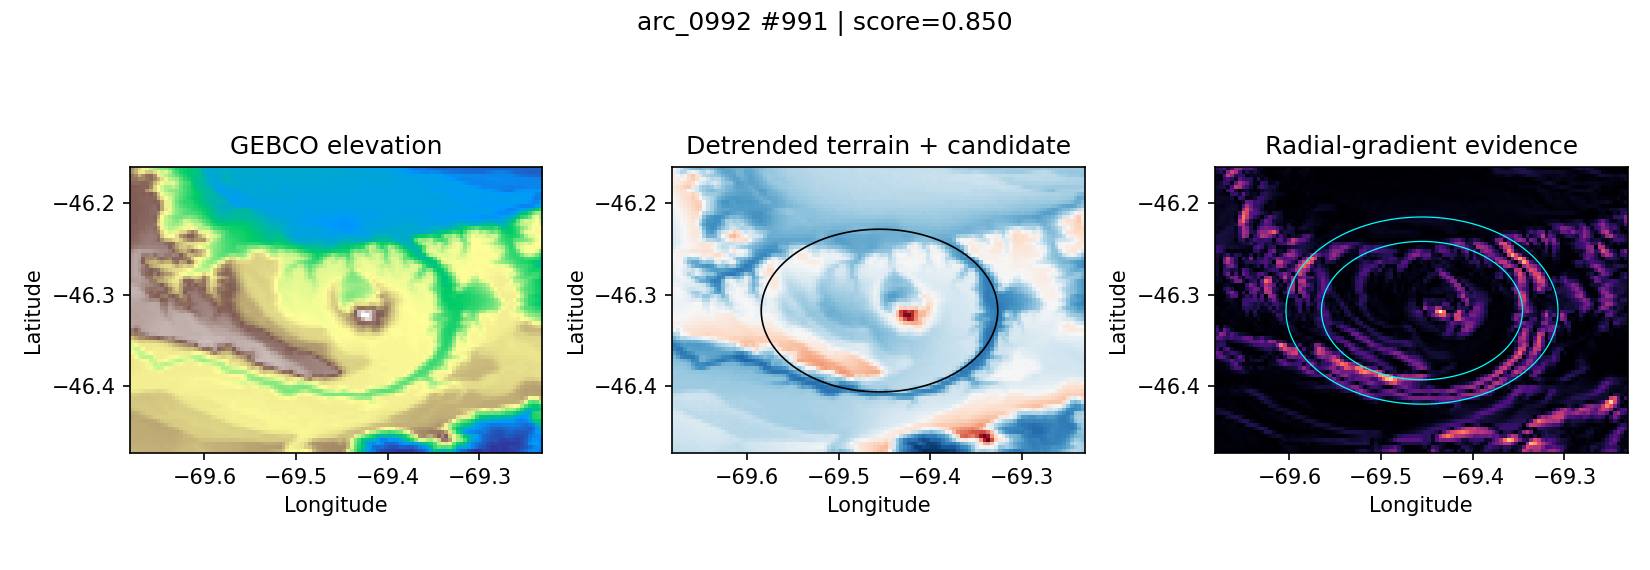
\includegraphics[width=0.98\textwidth]{ranking_output/diagnostics/arc_0992.png}
  \caption{Candidate \texttt{arc\_0992} at $46.317^{\circ}$S, $69.455^{\circ}$W. Its 20.0-km fitted geometry has morphology follow-up score 0.850 (rank 3) and a visually coherent radial-gradient response, but a gravity-consensus percentile of 0.286. It is consequently classified Tier C.}
  \label{fig:rank-0992}
\end{figure}

\begin{figure}[H]
  \centering
  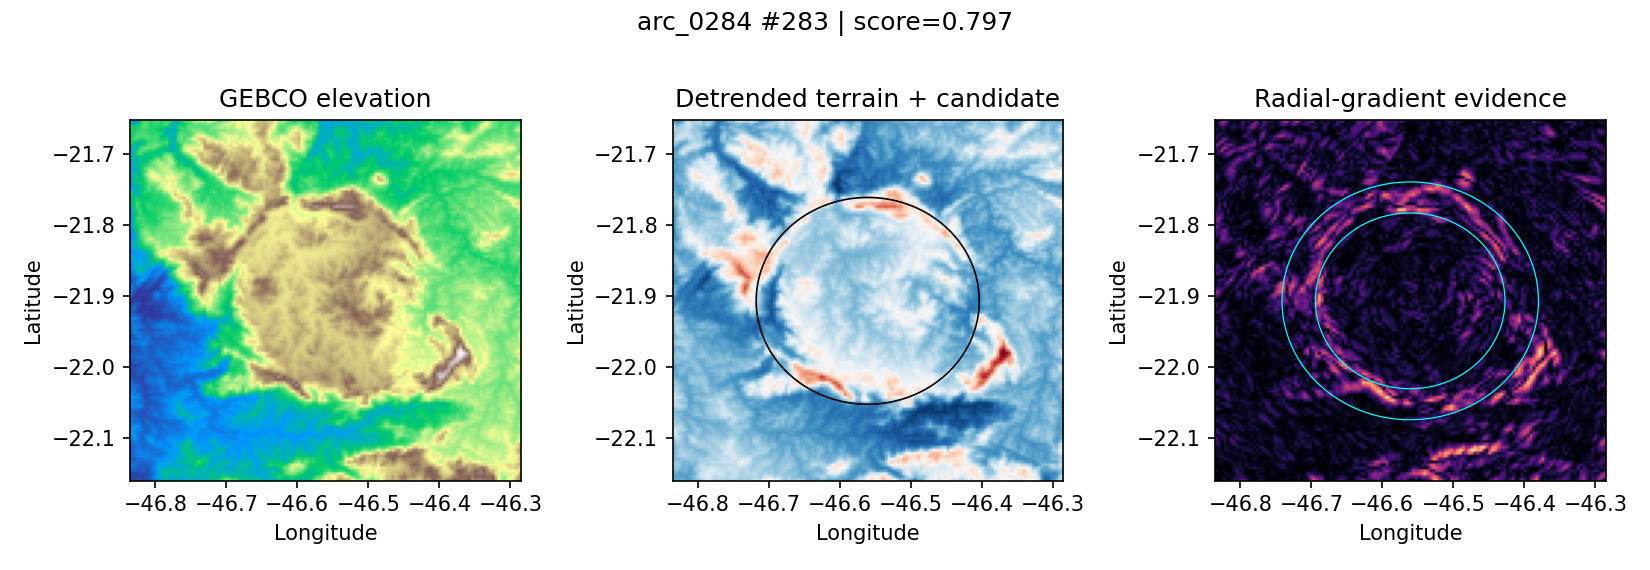
\includegraphics[width=0.98\textwidth]{ranking_output/diagnostics/arc_0284.png}
  \caption{Candidate \texttt{arc\_0284} at $21.907^{\circ}$S, $46.561^{\circ}$W. Its 32.6-km geometry has morphology follow-up score 0.797 (rank 21), with a comparatively continuous annular terrain-gradient pattern. Its gravity-consensus percentile is 0.370 and it remains Tier C pending independent geological and geophysical support.}
  \label{fig:rank-0284}
\end{figure}

\begin{thebibliography}{99}

\bibitem{French1998}
B. M. French, \emph{Traces of Catastrophe: A Handbook of Shock-Metamorphic Effects in Terrestrial Meteorite Impact Structures}, Lunar and Planetary Institute Contribution 954, 120~pp., 1998. Local source consulted: \dataset{CB-954.pdf}. \url{https://www.lpi.usra.edu/publications/books/CB-954/}

\bibitem{FrenchKoeberl2010}
B. M. French and C. Koeberl, ``The convincing identification of terrestrial meteorite impact structures: What works, what doesn't, and why,'' \emph{Earth-Science Reviews}, 98, 123--170, 2010. \url{https://doi.org/10.1016/j.earscirev.2009.10.009}

\bibitem{Gulick2013}
S. P. S. Gulick, G. L. Christeson, P. J. Barton, R. A. F. Grieve, J. V. Morgan and J. Urrutia-Fucugauchi, ``Geophysical characterization of the Chicxulub impact crater,'' \emph{Reviews of Geophysics}, 51, 31--52, 2013. \url{https://doi.org/10.1002/rog.20007}

\bibitem{Girdler1992}
R. W. Girdler, P. T. Taylor and J. J. Frawley, ``A possible impact origin for the Bangui magnetic anomaly (Central Africa),'' \emph{Tectonophysics}, 212, 45--58, 1992. Local source consulted: \dataset{A possible impact origin for the Bangui magnetic anomaly.pdf}.

\bibitem{Osinski2022}
G. R. Osinski et al., ``Impact Earth: A review of the terrestrial impact record,'' \emph{Earth-Science Reviews}, 232, 104112, 2022. \url{https://doi.org/10.1016/j.earscirev.2022.104112}

\bibitem{Potter2013}
R. W. K. Potter, D. A. Kring, G. S. Collins, W. S. Kiefer and P. J. McGovern, ``Numerical modeling of the formation and structure of the Orientale impact basin,'' \emph{Journal of Geophysical Research: Planets}, 118, 963--979, 2013. \url{https://doi.org/10.1002/jgre.20080}

\bibitem{ReimoldKoeberl2014}
W. U. Reimold and C. Koeberl, ``Impact structures in Africa: A review,'' \emph{Journal of African Earth Sciences}, 93, 57--175, 2014. \url{https://doi.org/10.1016/j.jafrearsci.2014.01.008}

\bibitem{Robbins2018}
S. J. Robbins et al., ``Revised recommended methods for analyzing crater size-frequency distributions,'' \emph{Meteoritics \& Planetary Science}, 53, 891--931, 2018. \url{https://doi.org/10.1111/maps.12990}

\bibitem{Robbins2019}
S. J. Robbins, ``A new global database of lunar impact craters $>1$--2~km: 1. Crater locations and sizes, comparisons with published databases, and global analysis,'' \emph{Journal of Geophysical Research: Planets}, 124, 871--892, 2019. \url{https://doi.org/10.1029/2018JE005592}

\bibitem{Neumann2015}
G. A. Neumann et al., ``Lunar impact basins revealed by Gravity Recovery and Interior Laboratory measurements,'' \emph{Science Advances}, 1, e1500852, 2015. \url{https://doi.org/10.1126/sciadv.1500852}

\bibitem{PikeSpudis1987}
R. J. Pike and P. D. Spudis, ``Basin-ring spacing on the Moon, Mercury, and Mars,'' \emph{Earth, Moon, and Planets}, 39, 129--194, 1987. \url{https://doi.org/10.1007/BF00054060}

\bibitem{Ryder2002}
G. Ryder, ``Mass flux in the ancient Earth--Moon system and benign implications for the origin of life on Earth,'' \emph{Journal of Geophysical Research: Planets}, 107(E4), 5022, 2002. \url{https://doi.org/10.1029/2001JE001583}

\bibitem{RyderKoeberlMojzsis2000}
G. Ryder, C. Koeberl and S. J. Mojzsis, ``Heavy bombardment of the Earth at approximately 3.85~Ga: The search for petrographic and geochemical evidence,'' in R. M. Canup and K. Righter (eds.), \emph{Origin of the Earth and Moon}, University of Arizona Press, 475--492, 2000. \url{https://doi.org/10.2307/j.ctv1v7zdrp.30}

\bibitem{FassettMinton2013}
C. I. Fassett and D. A. Minton, ``Impact bombardment of the terrestrial planets and the early history of the Solar System,'' \emph{Nature Geoscience}, 6, 520--524, 2013. \url{https://doi.org/10.1038/ngeo1841}

\bibitem{Marchi2024}
S. Marchi et al., ``Impact-generated permeability and hydrothermal circulation at the Vredefort impact structure, South Africa,'' \emph{Earth and Space Science}, 11, e2023EA003065, 2024. \url{https://doi.org/10.1029/2023EA003065}

\bibitem{Therriault1997}
A. M. Therriault, R. A. F. Grieve and W. U. Reimold, ``Original size of the Vredefort Structure: Implications for the geological evolution of the Witwatersrand Basin,'' \emph{Meteoritics \& Planetary Science}, 32, 71--77, 1997. \url{https://doi.org/10.1111/j.1945-5100.1997.tb01242.x}

\bibitem{Torrese2022}
P. Torrese, ``Subsurface structure of the proposed Sirente meteorite crater: insights from ERT synthetic modelling,'' \emph{Acta Geodaetica et Geophysica}, 57, 563--587, 2022. \url{https://doi.org/10.1007/s40328-022-00391-7}

\bibitem{StyronPagani2020}
R. Styron and M. Pagani, ``The GEM Global Active Faults Database,'' \emph{Earthquake Spectra}, 36(S1), 160--180, 2020. \url{https://doi.org/10.1177/8755293020944182}

\bibitem{GEBCO2026}
GEBCO Compilation Group, \emph{GEBCO 2026 Grid}, 15-arcsecond global terrain model and Type Identifier grid, 2026. \url{https://doi.org/10.5285/4f68d5c7-45eb-f999-e063-7086abc036fa}

\bibitem{Bonvalot2012}
S. Bonvalot et al., \emph{World Gravity Map}, Bureau Gravim\'etrique International, CGMW--BGI--CNES--IRD, Paris, 2012.

\bibitem{Balmino2012}
G. Balmino, N. Vales, S. Bonvalot and A. Briais, ``Spherical harmonic modelling to ultra-high degree of Bouguer and isostatic anomalies,'' \emph{Journal of Geodesy}, 86, 499--520, 2012. \url{https://doi.org/10.1007/s00190-011-0533-4}

\bibitem{Meyer2017}
B. Meyer, A. Chulliat and R. Saltus, ``Derivation and error analysis of the Earth Magnetic Anomaly Grid at 2 arc min resolution version 3 (EMAG2v3),'' \emph{Geochemistry, Geophysics, Geosystems}, 18, 4522--4537, 2017. \url{https://doi.org/10.1002/2017GC007280}

\bibitem{Straume2019}
E. O. Straume et al., ``GlobSed: Updated total sediment thickness in the world's oceans,'' \emph{Geochemistry, Geophysics, Geosystems}, 20, 1756--1772, 2019. \url{https://doi.org/10.1029/2018GC008115}

\bibitem{Laske2013}
G. Laske, G. Masters, Z. Ma and M. Pasyanos, ``Update on CRUST1.0---A 1-degree global model of Earth's crust,'' EGU General Assembly 2013, abstract EGU2013-2658, 2013.

\end{thebibliography}

\end{document}
